\chapter{Dimensionality Reduction}

The \textbf{curse of dimensionality} makes multivariate data hard both to \emph{visualize} and to \emph{extract useful information from}. Dimensionality Reduction tackles this problem by ``\emph{solving problems by changing the viewpoint}'': it automatically finds good features by learning a hypothesis map that reads the representation of a data point and transforms it into a smaller set of features. The aim is to obtain a \textbf{compressed representation} of the data. Note that, in this sense, feature engineering also means \textbf{feature reduction}.

Reducing the number of features is good practice because it allows to:

\begin{itemize}
    \item Capture the important information in a dataset more efficiently than the original attributes.
    \item Visualize data more easily.
    \item Reduce \underline{overfitting}, improving the generalization of models.
    \item Avoid the curse of dimensionality.
    \item Reduce the time and memory required by algorithms.
    \item Eliminate irrelevant features and reduce noise.
\end{itemize}

The main techniques are: Singular Value Decomposition (SVD), Principal Component Analysis (PCA), Linear Discriminant Analysis (LDA) and non-linear techniques (e.g.\ Kernel PCA, t-SNE).

\begin{figure}[h]
    \centering
    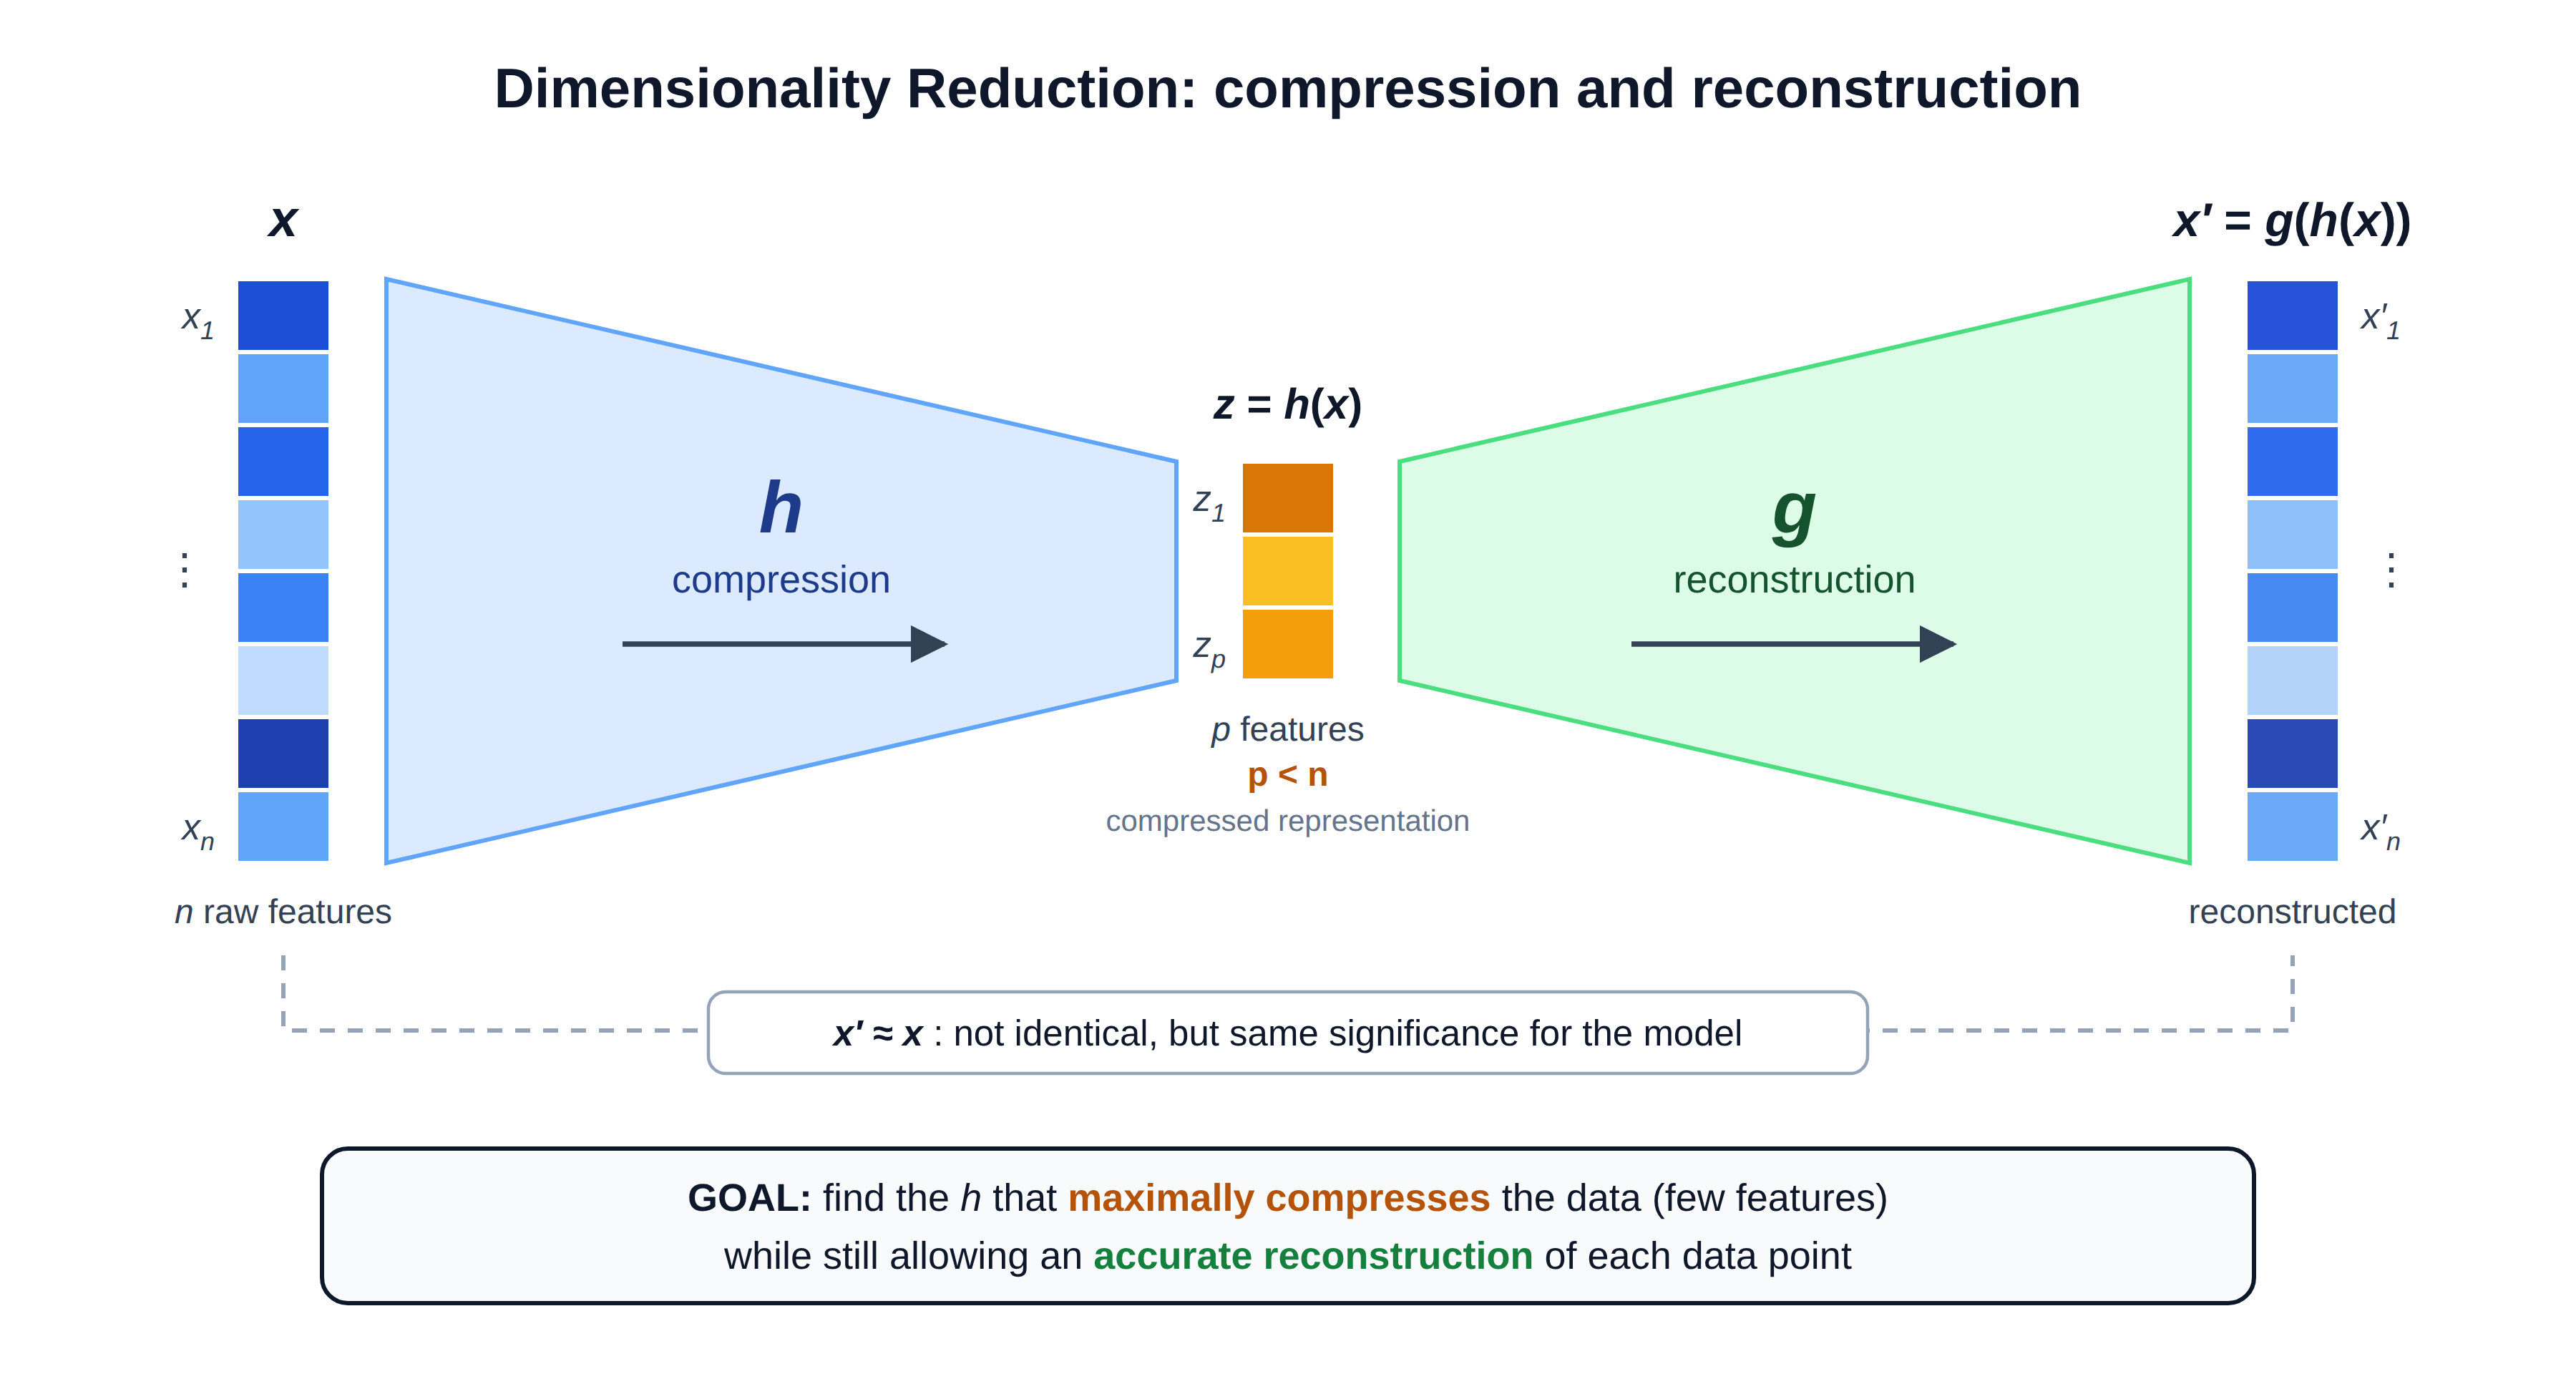
\includegraphics[width=0.6\textwidth]{images/chapter_4/dr_compression_reconstruction.png}
    \caption{Compression map $h$ and reconstruction map $g$}
\end{figure}

Every Dimensionality Reduction process is built around two maps:

\begin{itemize}
    \item \textbf{Compression}: a map $h$ that goes from $n$ raw features to $p$ features ($p < n$), producing the compressed representation $z = h(x)$.
    \item \textbf{Reconstruction}: a map $g$ that recovers the original values from the compressed ones, $x' = g(h(x))$. The reconstructed $x'$ is not exactly equal to $x$, but very similar, i.e.\ it carries the same significance with respect to the model.
    \item \textbf{Goal}: find the $h$ that \emph{maximally compresses} the raw data while still allowing an \emph{accurate reconstruction} of each data point from a small number of features.
\end{itemize}

\section{PCA: Principal Component Analysis}
PCA was introduced by Pearson and Hotelling to describe the variation in a set of multivariate data in terms of a set of \textbf{uncorrelated} variables. We start from a data matrix $X$ ($m \times n$): each \emph{row} is an observation (a data point), each \emph{column} is one of the $n$ correlated variables $x_1, x_2, \dots, x_n$. PCA transforms them into $p \le n$ new variables $x'_i$ that are \textbf{uncorrelated}. To do so it builds a \textbf{new basis} (a new set of axes) in which the \textbf{first axis carries the maximum information} about the data. For PCA, information means \textbf{variance}: a direction along which the data are very spread out tells us a lot, while a direction along which all points are almost equal tells us almost nothing.

PCA is useful when there is \textbf{redundancy} in the variables, i.e.\ when the \textbf{data do not span the whole $n$-dimensional space}. Redundancy means that some variables are \textbf{correlated}: if $x_2$ almost always grows with $x_1$, the two variables largely carry the same information. Because of it, the observed variables can be summarized by a \textbf{smaller number of principal components} that still account for \textbf{most of the variance}.

\begin{figure}[h]
    \centering
    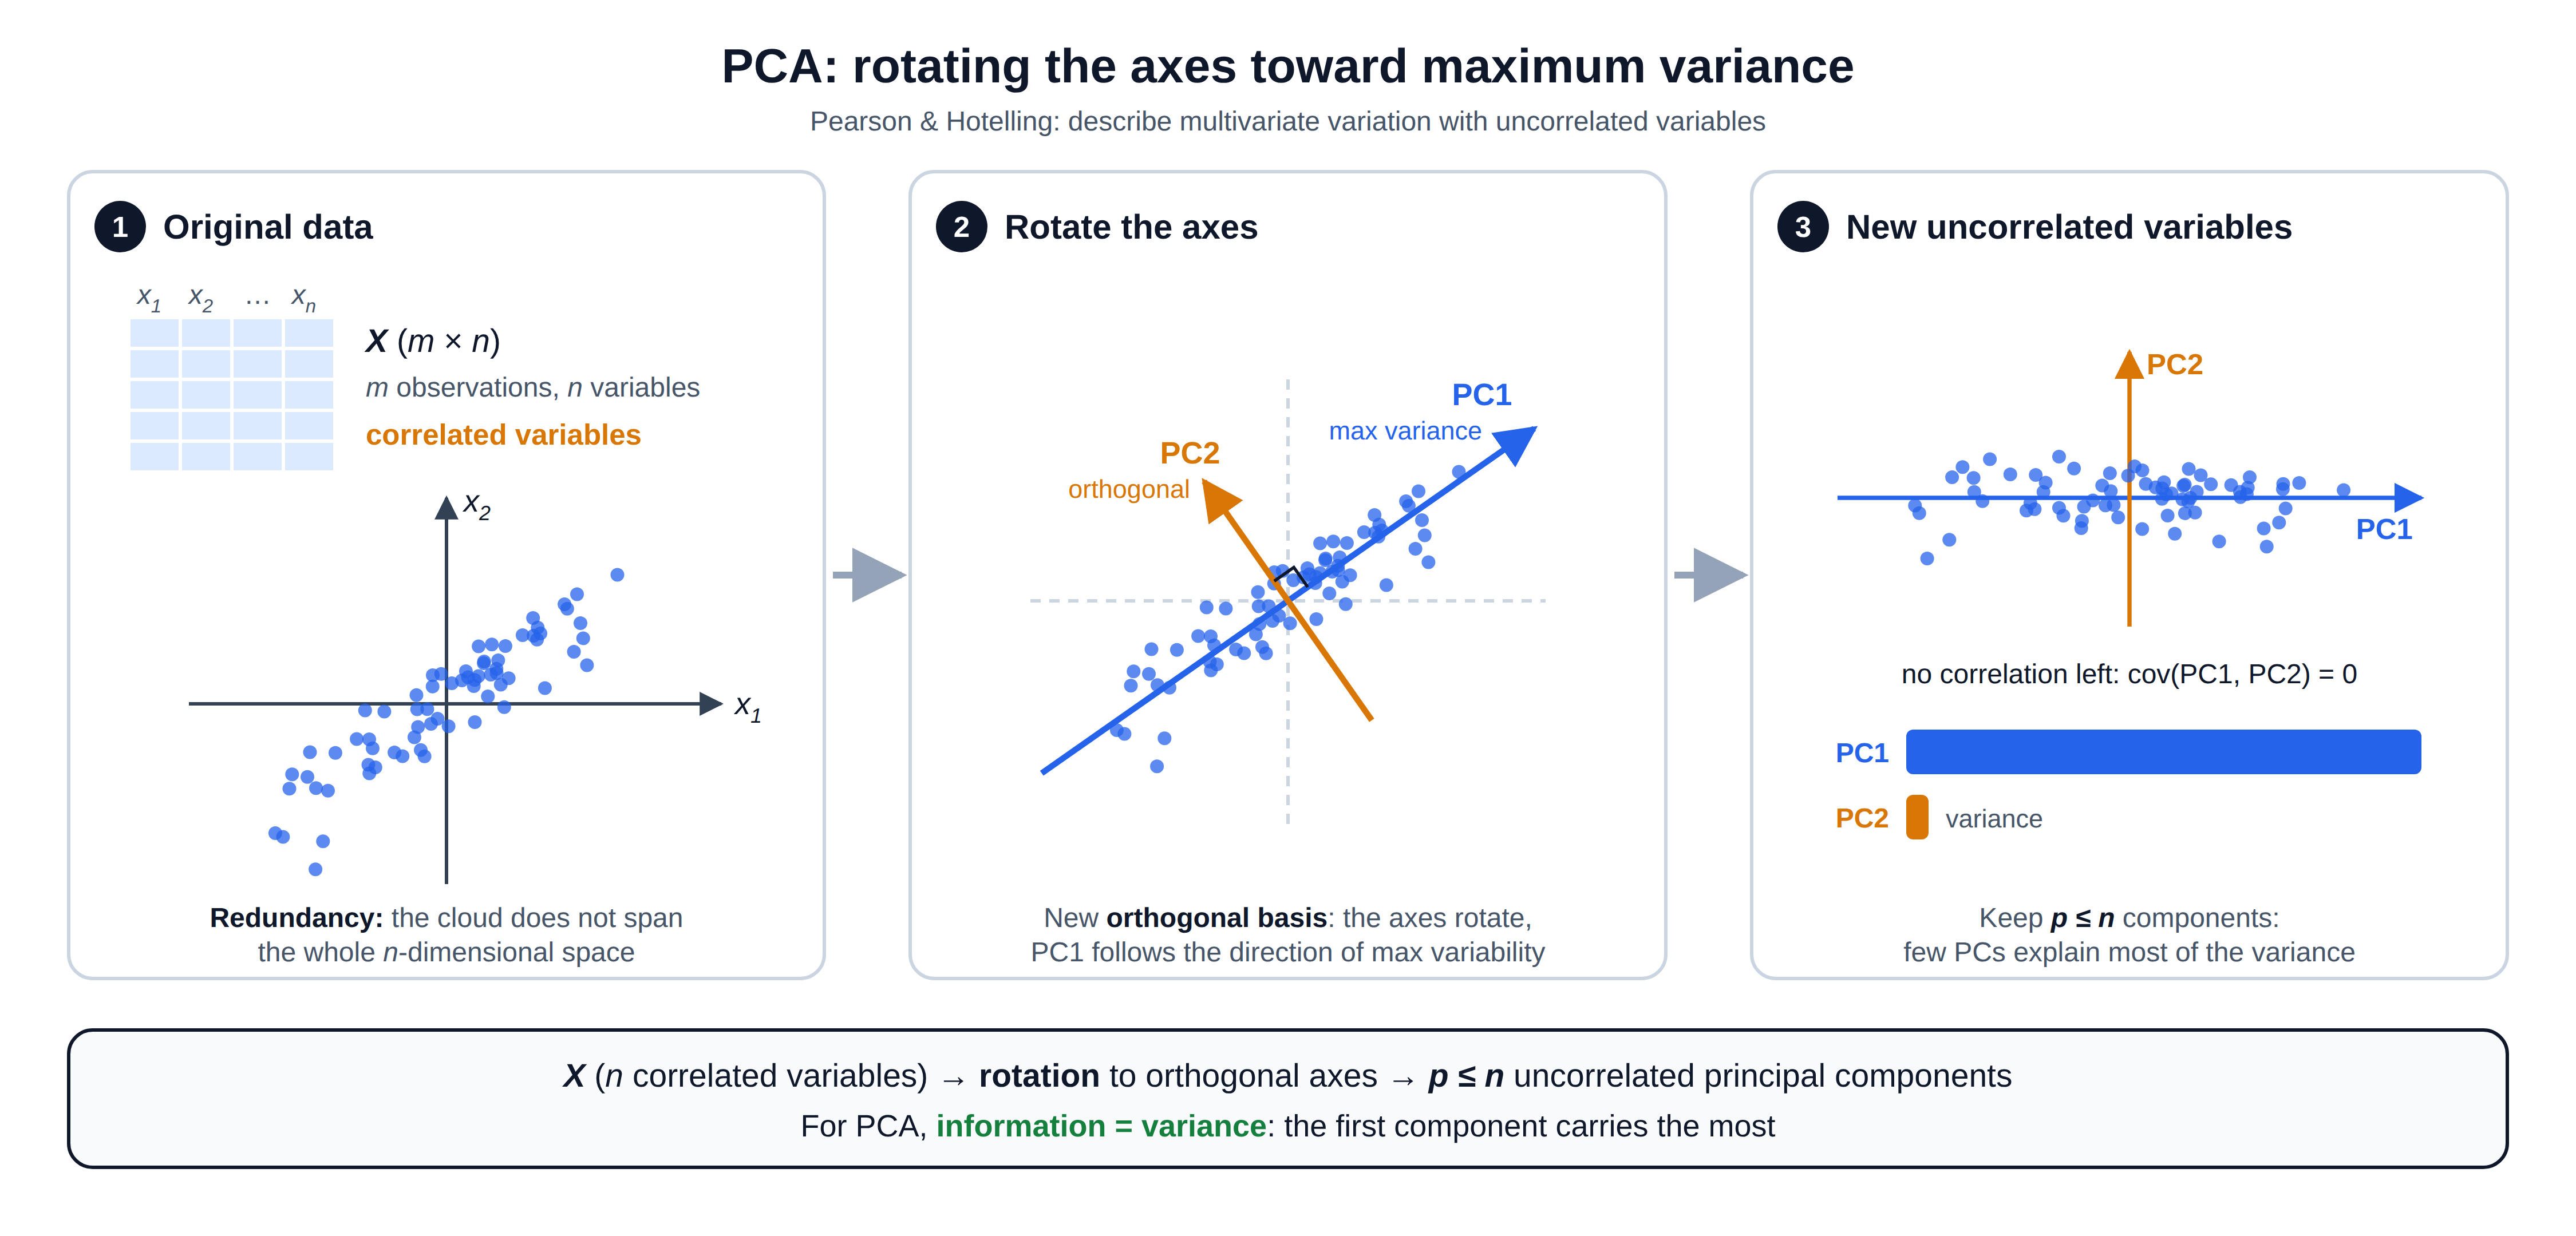
\includegraphics[width=1\textwidth]{images/chapter_4/pca_rotation_axes.png}
    \caption{PCA as a rotation of the axes toward maximum variance}
\end{figure}

In a nutshell, PCA is a \textbf{rotation of the existing axes}. The data points do not move; we only look at them from a new viewpoint. The new axes are \textbf{orthogonal} and point in the directions of \underline{maximum variability}.

\subsection{PCA: Definition}
PCA has two equivalent definitions (see the figure below: data points in red, principal subspace in magenta, projection errors in blue):

\begin{itemize}
    \item \textbf{Maximum variance}: find a lower-dimensional space, called the \emph{principal subspace}, such that the orthogonal projections of the data points onto it are \textbf{as spread out as possible}, i.e.\ have \textbf{maximum variance}.
    \item \textbf{Minimum error}: find the subspace that \textbf{minimizes the sum of the squared projection errors}, i.e.\ of the squared distances of the points from the new axis.
\end{itemize}

\textbf{Why are they equivalent?} For each point, the distance from the mean is fixed and, by Pythagoras, $\text{distance}^2 = \text{projection}^2 + \text{error}^2$. Since the left side does not depend on the chosen axis, \emph{making the projections as long as possible} is the same as \emph{making the errors as short as possible}. The error is exactly what we lose when we rebuild $x'$ from its projection. So PCA also \textbf{minimizes the reconstruction error} between $x'$ and $x$, and can be seen either as a maximization or as a minimization problem.

\begin{figure}[h]
    \centering
    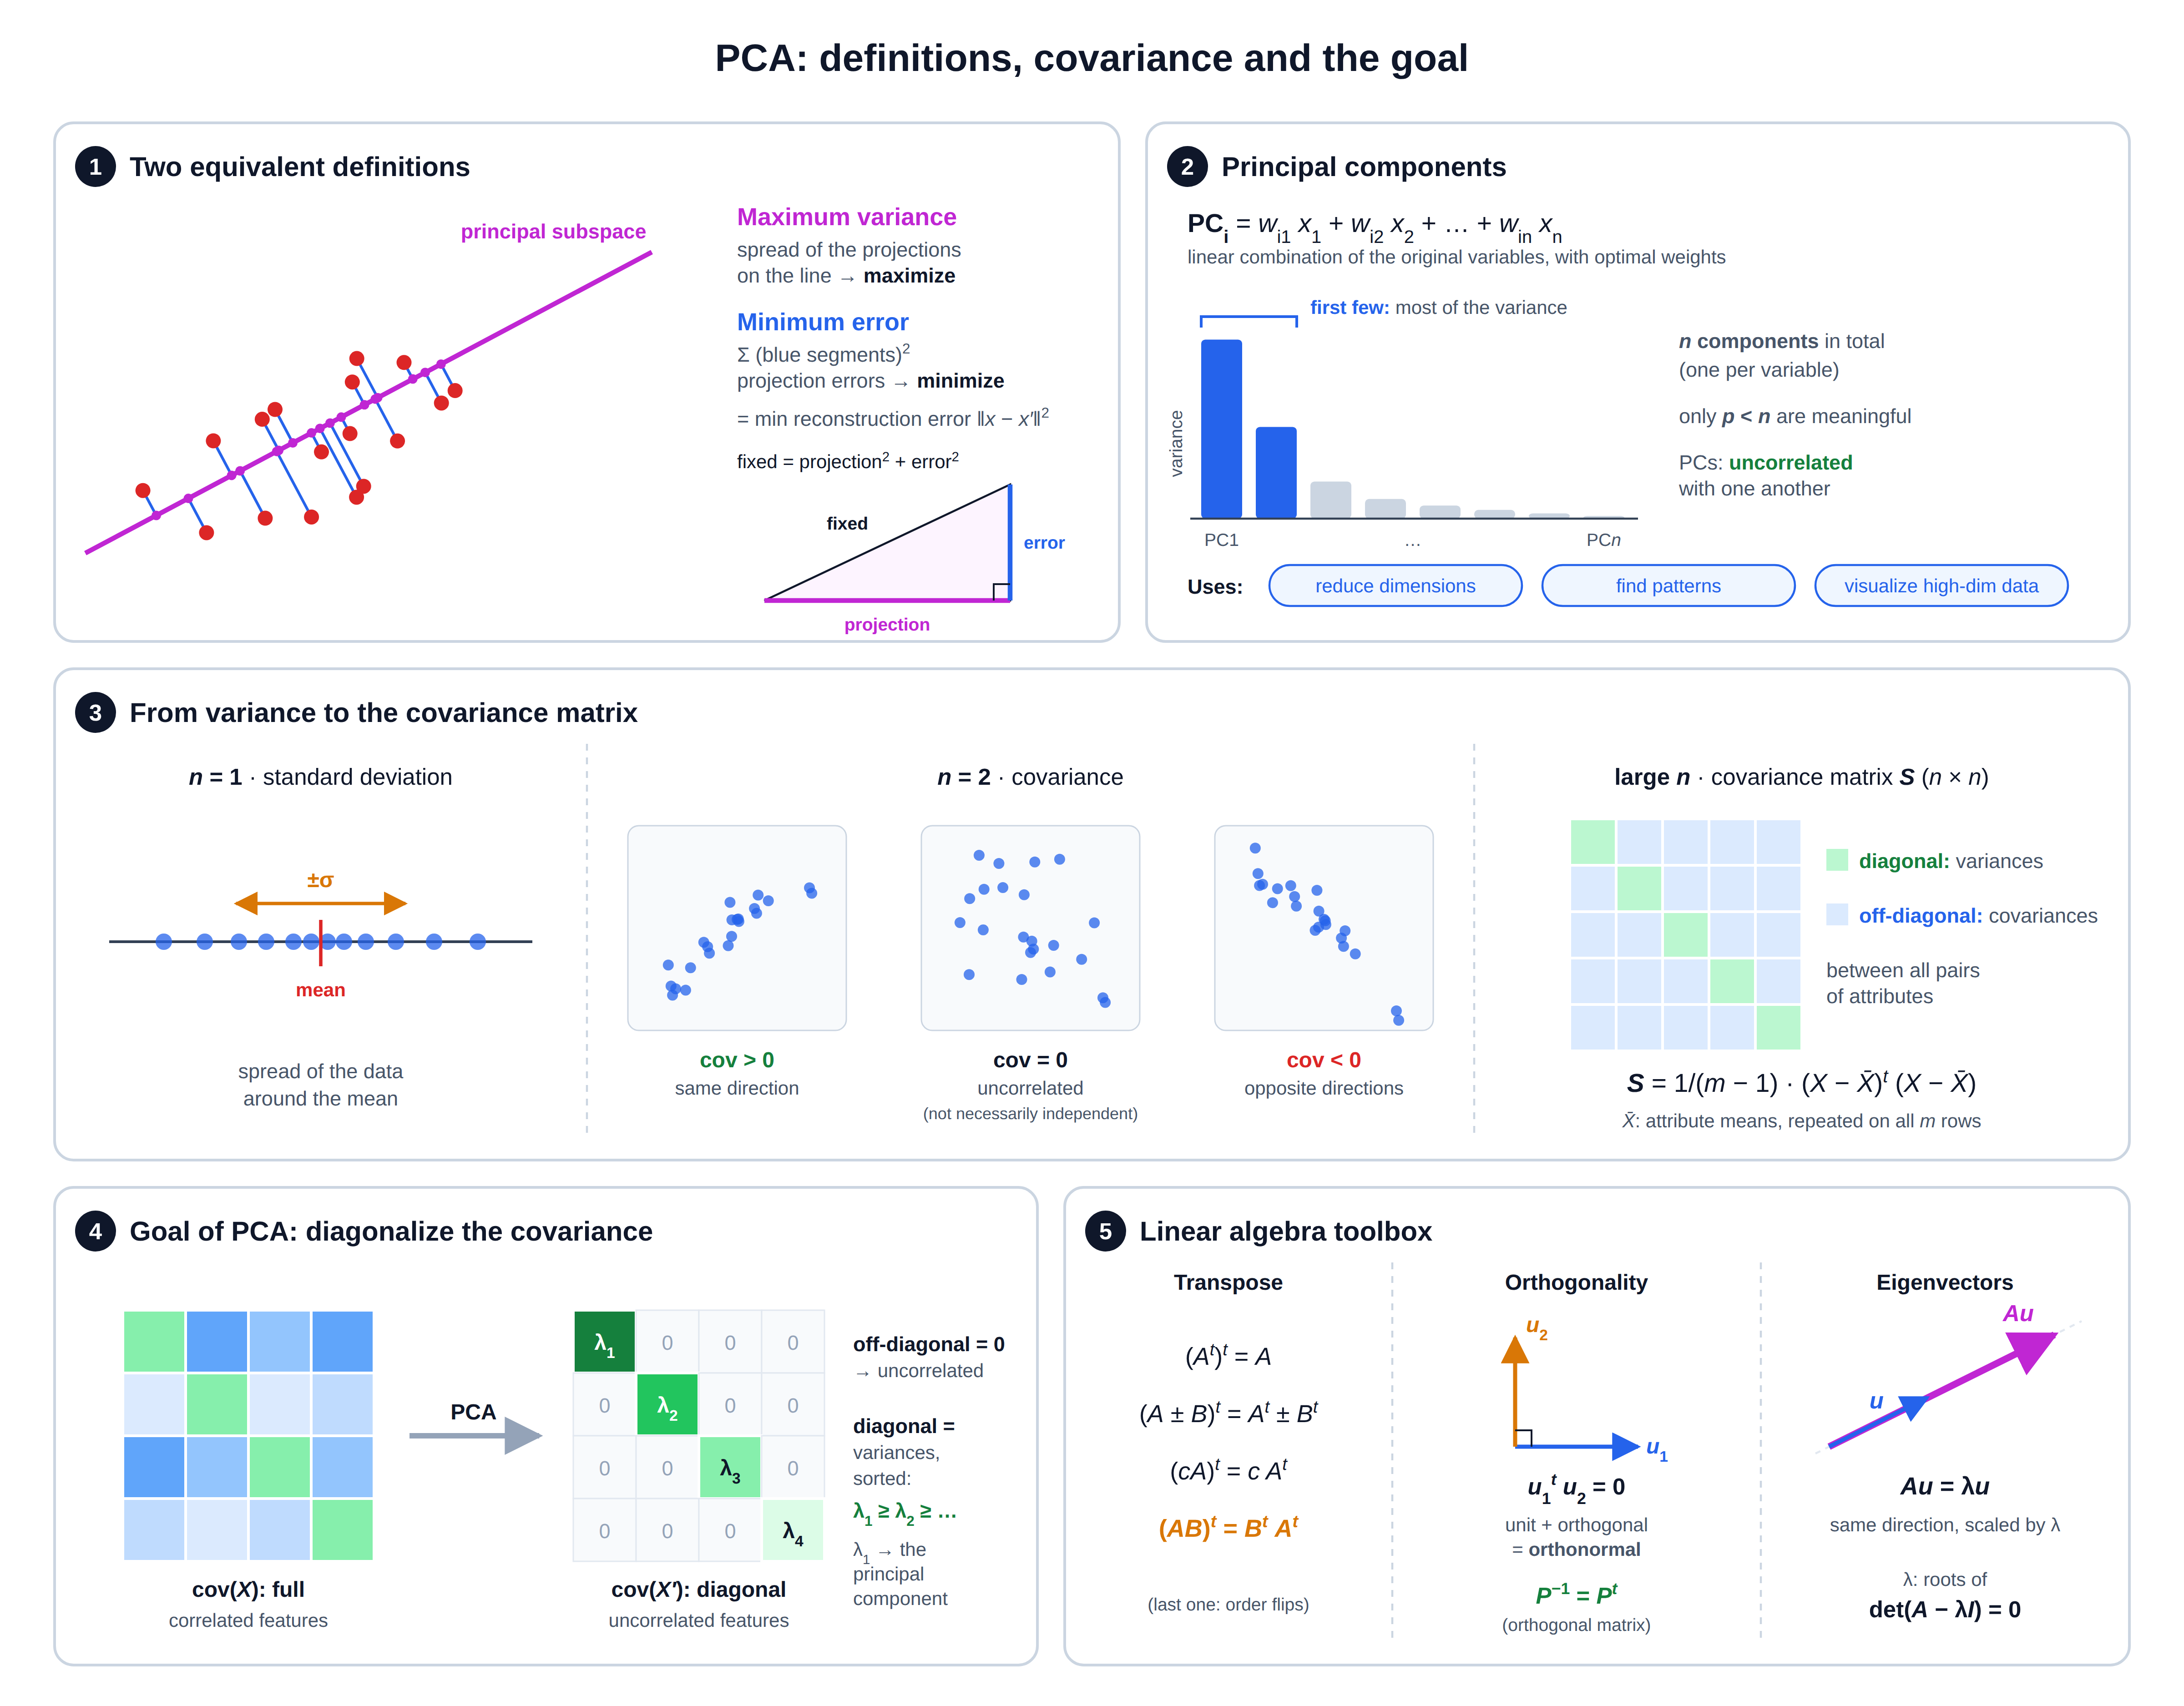
\includegraphics[width=1\textwidth]{images/chapter_4/pca_definitions_covariance.png}
    \caption{PCA definitions, from variance to covariance, and linear algebra remarks}
\end{figure}

A Principal Component is a \textbf{linear combination} of the observed variables with optimal weights:
\[
    \text{PC}_i = w_{i1}x_1 + w_{i2}x_2 + \dots + w_{in}x_n
\]
The weight vector $(w_{i1}, \dots, w_{in})$ is the \emph{direction} of the $i$-th new axis. As many components can be extracted as there are variables ($n$), but usually only the \textbf{first few account for a meaningful amount of variance} ($p < n$). Each component is correlated, to varying degrees, with some of the original variables (those with large weights). However, the components are \textbf{completely uncorrelated with one another}.

PCA can be used to:
\begin{itemize}
    \item Reduce the number of dimensions in data.
    \item Find patterns in high-dimensional data.
    \item Visualize high-dimensional data.
\end{itemize}

\paragraph{From variance to the covariance matrix.}
To find the directions of maximum variance, we first need a tool that describes how the data vary along \emph{every} direction:
\begin{itemize}
    \item With a single attribute ($n=1$), the \textbf{standard deviation} (or its square, the variance) measures how far the data are spread around the mean.
    \item With two attributes ($n=2$), the \textbf{covariance} measures how $x$ and $y$ vary together. If $\operatorname{cov}(x,y) > 0$ they move in the same direction, and if $\operatorname{cov}(x,y) < 0$ they move in opposite directions. If $\operatorname{cov}(x,y) = 0$ they are \emph{uncorrelated}: there is no linear relationship, though they are not necessarily independent.
    \item For a large $n$, all this information is collected in the \textbf{covariance matrix}. It has the variance of each attribute on the diagonal and the covariance of each pair of attributes off the diagonal.
\end{itemize}

\begin{figure}[h!]
    \centering
    \begin{minipage}{0.8\textwidth}
    The sample covariance matrix $S$ ($n \times n$) of $X$ ($m \times n$) is:
    \[
        S = \frac{1}{m-1} (X - \overline{X})^t (X - \overline{X})
    \]
    where $\overline{X}$ is the $m \times n$ matrix of the attribute means: all its $m$ rows are equal to the mean of the rows of $X$. For example, with $n=2$:
    \[
        S = \begin{pmatrix} \operatorname{var}(x_1) & \operatorname{cov}(x_1,x_2) \\ \operatorname{cov}(x_2,x_1) & \operatorname{var}(x_2) \end{pmatrix}
    \]
    $S$ is always \textbf{symmetric}, since $\operatorname{cov}(x_1,x_2) = \operatorname{cov}(x_2,x_1)$.
    \end{minipage}
    \caption{Covariance Matrix}
\end{figure}

\begin{figure}[h]
    \centering
    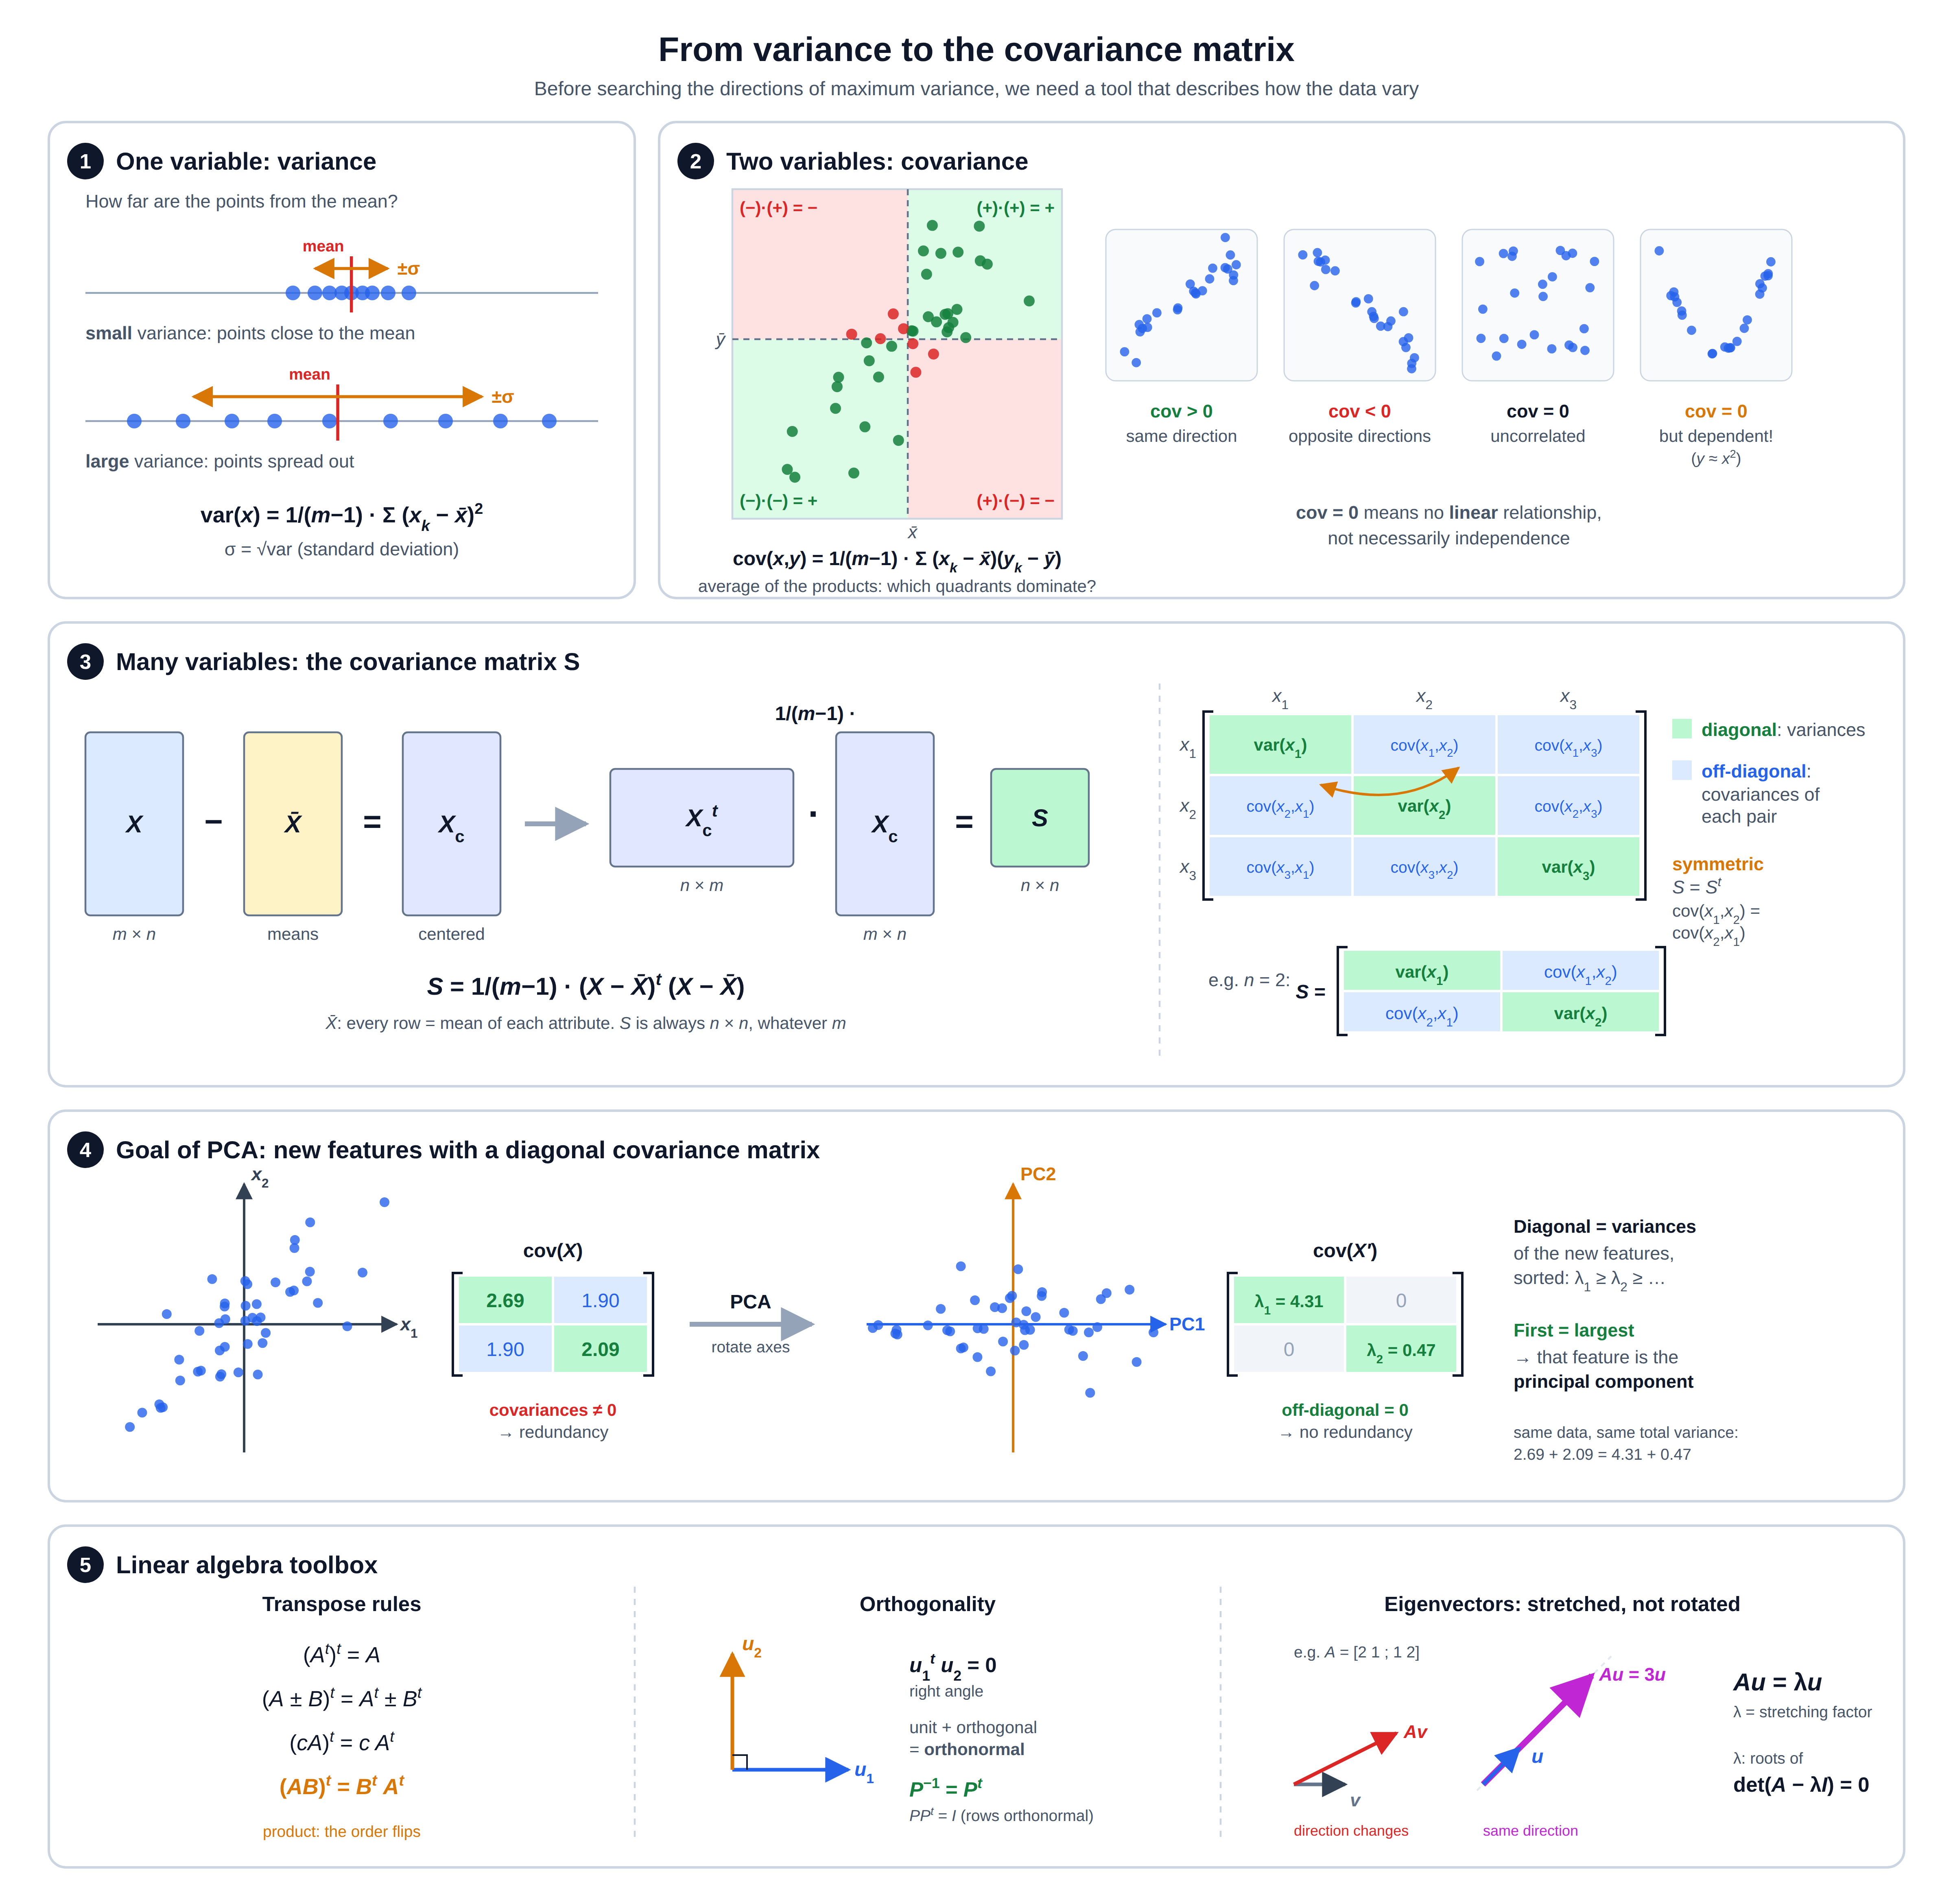
\includegraphics[width=1\textwidth]{images/chapter_4/covariance_matrix_explained.png}
    \caption{From variance to the covariance matrix, the goal of PCA and linear algebra remarks}
\end{figure}

\textbf{Goal of PCA}: find new features whose covariance matrix is \textbf{diagonal}:
\begin{itemize}
    \item off-diagonal entries equal to 0 mean the new features are pairwise uncorrelated, so there is no redundancy left;
    \item the diagonal holds their variances, sorted so that the \textbf{first one is the largest possible}; that feature is the principal component.
\end{itemize}

Useful matrix remarks:

\begin{figure}[h!]
    \centering
    \begin{minipage}{0.6\textwidth}
    If $A$ and $B$ are matrices whose sizes make the operations defined, and $c$ is any scalar:
    \begin{align*}
        (A^t)^t &= A \\
        (A \pm B)^t &= A^t \pm B^t \\
        (cA)^t &= cA^t \\
        (AB)^t &= B^t A^t
    \end{align*}
    \end{minipage}
    \caption{Matrix Remarks}
\end{figure}

Orthogonality and eigenvalue remarks:

\begin{itemize}
    \item Two vectors $u_1$ and $u_2$ are \textbf{orthogonal} if $u_1^t u_2 = 0$ (they form a right angle).
    \item Orthogonal unit vectors are called \textbf{orthonormal}.
    \item A matrix whose rows are orthonormal is \textbf{orthogonal}, and its inverse is its transpose: $P^{-1} = P^t$, i.e.\ $PP^t = I$.
    \item Vectors $u$ such that $Au$ has the same direction as $u$ are the \textbf{eigenvectors} of $A$: the matrix only stretches them, without rotating them.
    \item In $Au = \lambda u$, the stretching factor $\lambda$ is the corresponding \textbf{eigenvalue} of $A$.
    \item The eigenvalues are the roots of $\det(A - \lambda I) = 0$.
\end{itemize}

\section{PCA: orthonormal change of basis P}

\paragraph{What does a change of basis mean?}
Let $u$ be a unit vector representing a new axis. The coordinate of a data point $x$ along that axis is its \textbf{projection}, i.e.\ the dot product of $x$ and $u$. If we stack the $n$ new axes $u_1, \dots, u_n$ as the \emph{rows} of a matrix $P$, all the projections are computed at once:
\[
    X' = XP^t \qquad \text{entry } (i,j) \text{ of } X' = \text{coordinate of point } i \text{ along axis } u_j
\]
$X'$ contains the \emph{same points} as $X$, only described in the new coordinate system. PCA must therefore:

\begin{itemize}
    \item Choose an \textbf{orthonormal} basis $P$, i.e.\ new axes that are perpendicular unit vectors, so that the transformation is a pure rotation.
    \item Choose it so that $\operatorname{cov}(X')$ is \textbf{diagonal}, i.e.\ the new variables are uncorrelated.
    \item Keep the first $p$ rows of $P$ as the \textbf{principal components} of $X$.
\end{itemize}

\begin{figure}[h]
    \centering
    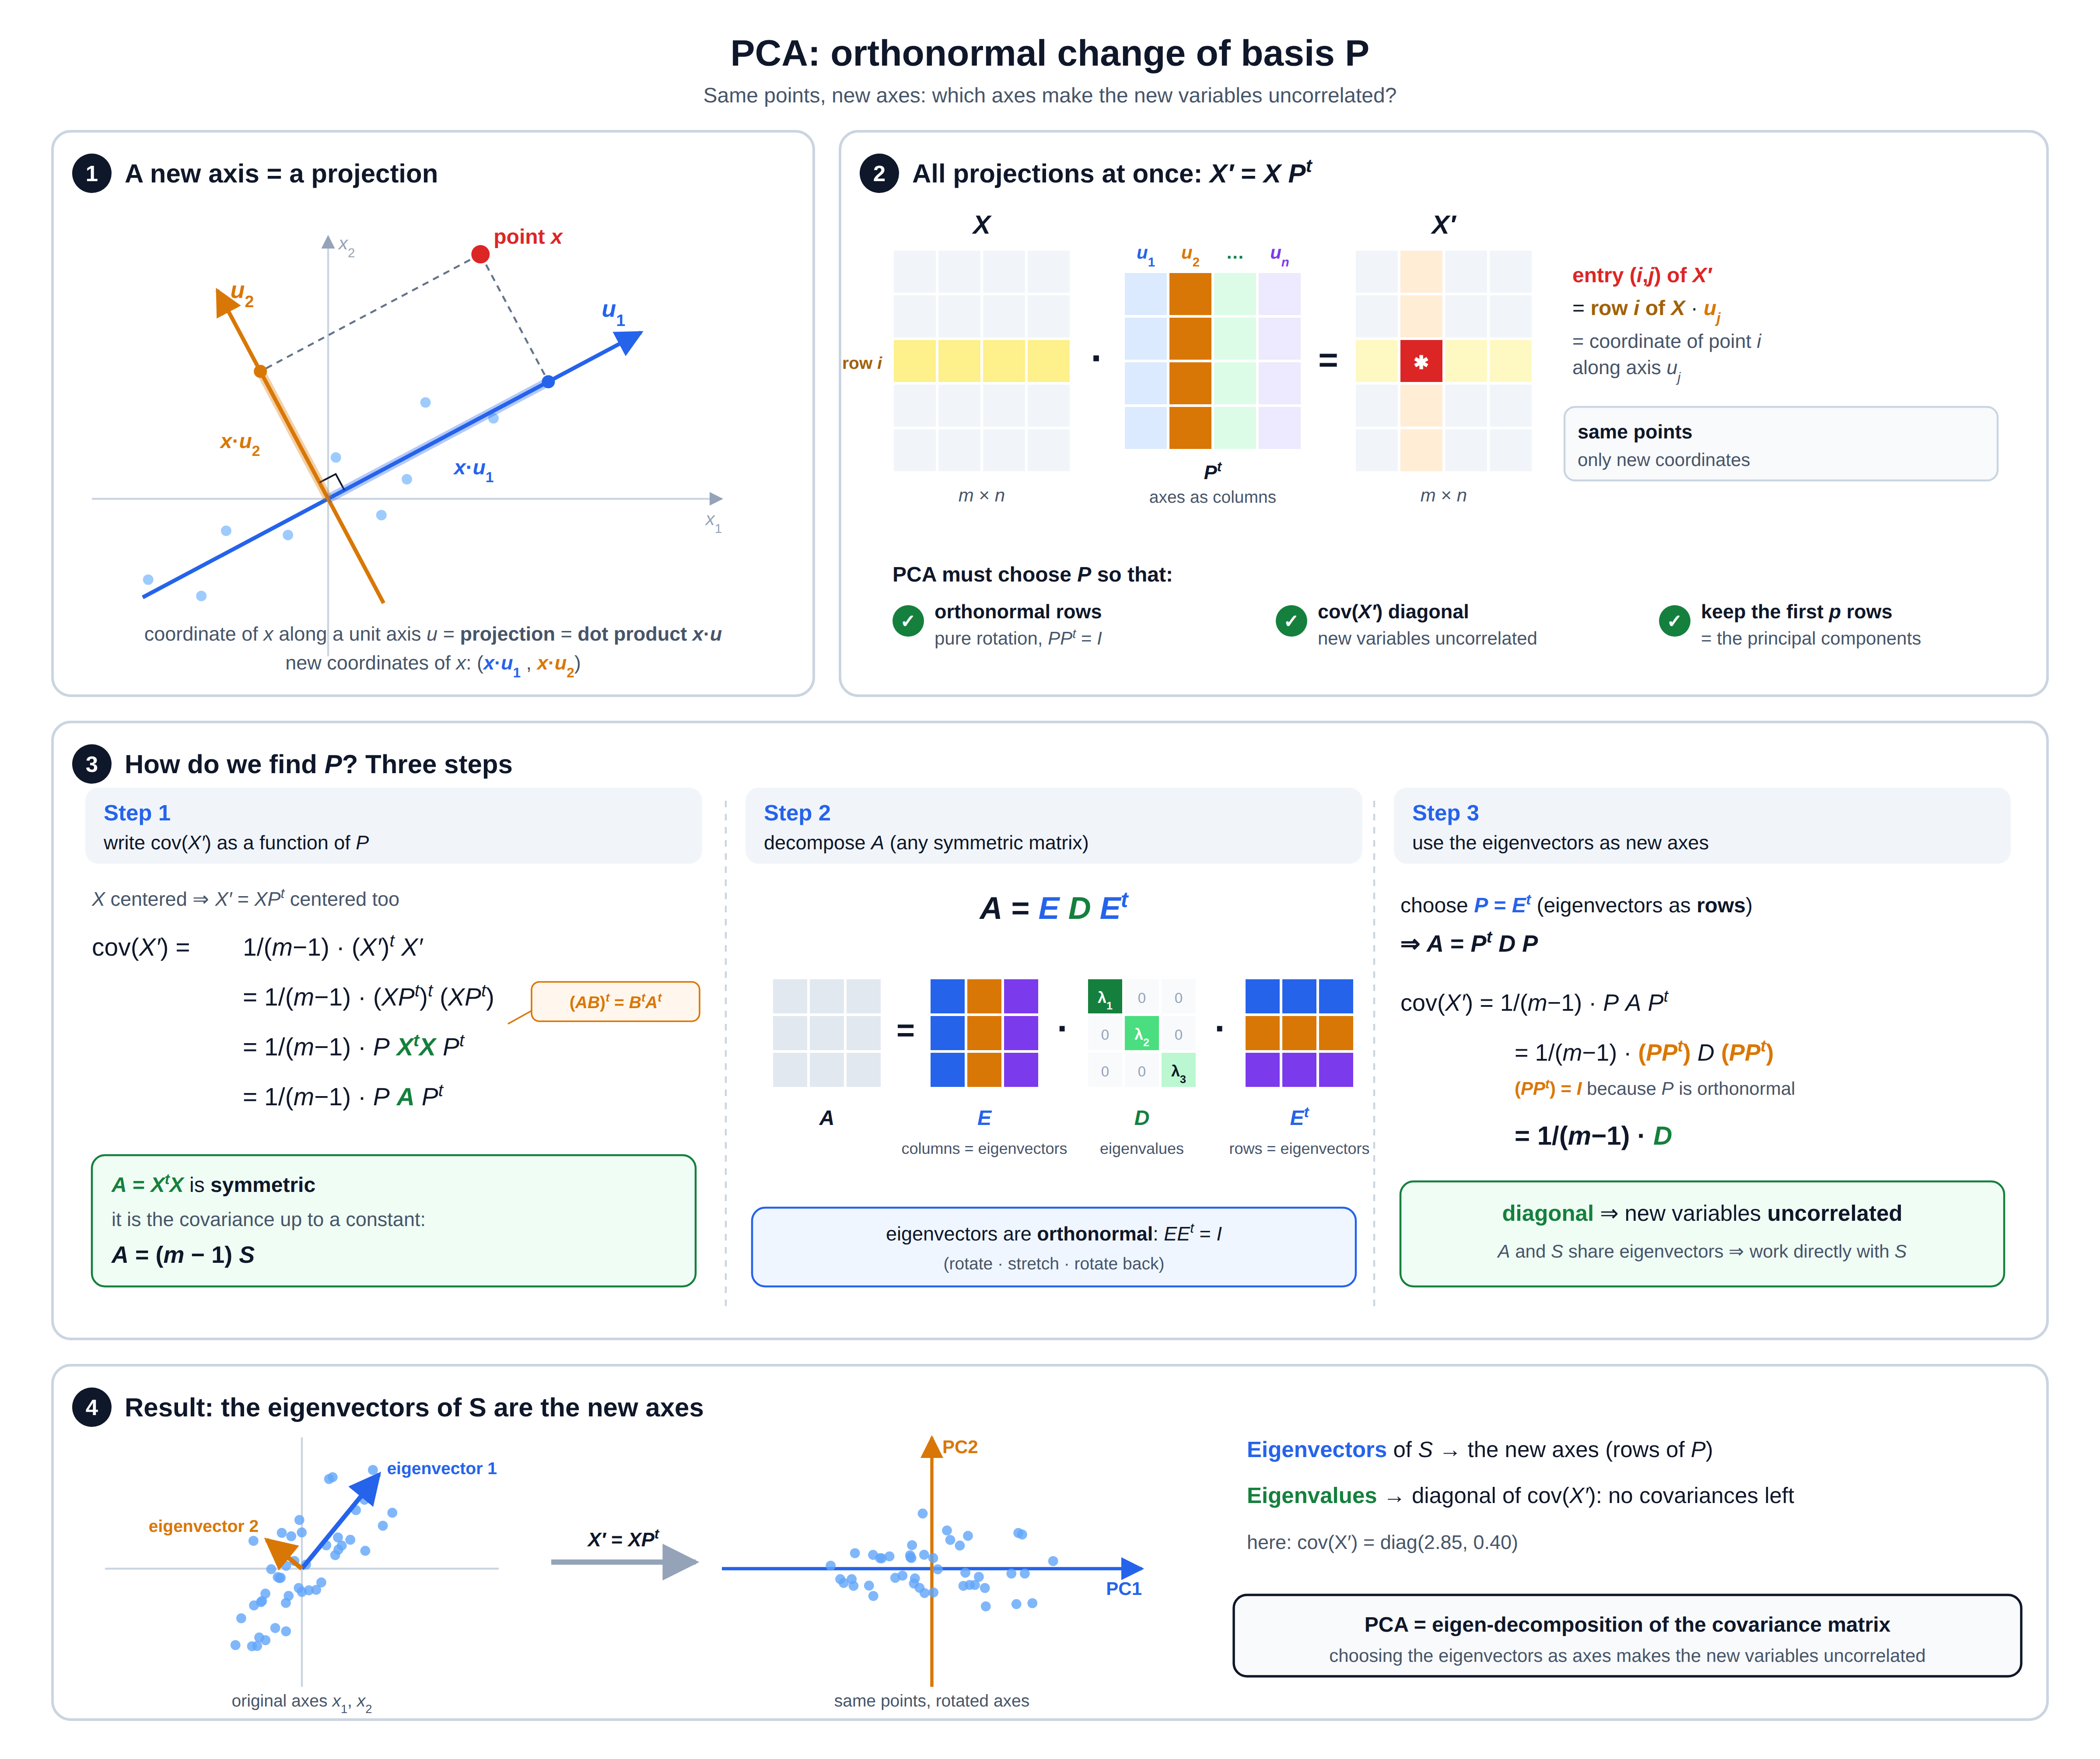
\includegraphics[width=1\textwidth]{images/chapter_4/pca_change_of_basis.png}
    \caption{Change of basis $X' = XP^t$ and why the eigenvectors diagonalize $\operatorname{cov}(X')$}
\end{figure}

\textbf{How do we find such a $P$?}

\textbf{Step 1: write $\operatorname{cov}(X')$ as a function of $P$.} Assume $X$ is centered (zero mean); then $X' = XP^t$ is centered too, and its covariance is simply $\frac{1}{m-1}(X')^tX'$. Substituting $X' = XP^t$ and using $(AB)^t = B^tA^t$:
\[
    \operatorname{cov}(X') = \frac{1}{m-1} (XP^t)^t (XP^t) = \frac{1}{m-1} P \,\underbrace{X^t X}_{A}\, P^t = \frac{1}{m-1} P A P^t
\]
The matrix $A = X^tX$ is \textbf{symmetric} and is just the covariance of the original data up to a constant: $A = (m-1)S$.

\textbf{Step 2: decompose $A$.} Every symmetric matrix can be written as
\[
    A = E D E^t
\]
where the columns of $E$ are the (orthonormal) \textbf{eigenvectors} of $A$ and $D$ is the diagonal matrix of its \textbf{eigenvalues}.

\textbf{Step 3: choose the eigenvectors as new axes.} Set $P = E^t$, so that the eigenvectors become the \emph{rows} of $P$. Then $A = P^t D P$ and, since $PP^t = I$:
\[
    \operatorname{cov}(X') = \frac{1}{m-1} \underbrace{P P^t}_{I} D \underbrace{P P^t}_{I} = \frac{1}{m-1} D
\]
which is \textbf{diagonal}. Therefore, using the eigenvectors as new axes makes the new variables uncorrelated. Since $A$ and $S$ differ only by a constant, they have the same eigenvectors, so in practice we work directly with $S$.

\paragraph{Why do the eigenvalues give the variance?}
The variance of the (centered) data projected on a unit vector $u$ is
\[
    \operatorname{var}(Xu) = \frac{1}{m-1}(Xu)^t(Xu) = u^t S u
\]
If $u$ is an eigenvector of $S$ ($Su = \lambda u$), this becomes $u^t \lambda u = \lambda$, because $u^tu = 1$. So \textbf{each eigenvalue is the variance of the data along its eigenvector}. The direction with the largest variance is therefore the eigenvector with the largest eigenvalue (the formal proof of the maximization is omitted).

\begin{figure}[h]
    \centering
    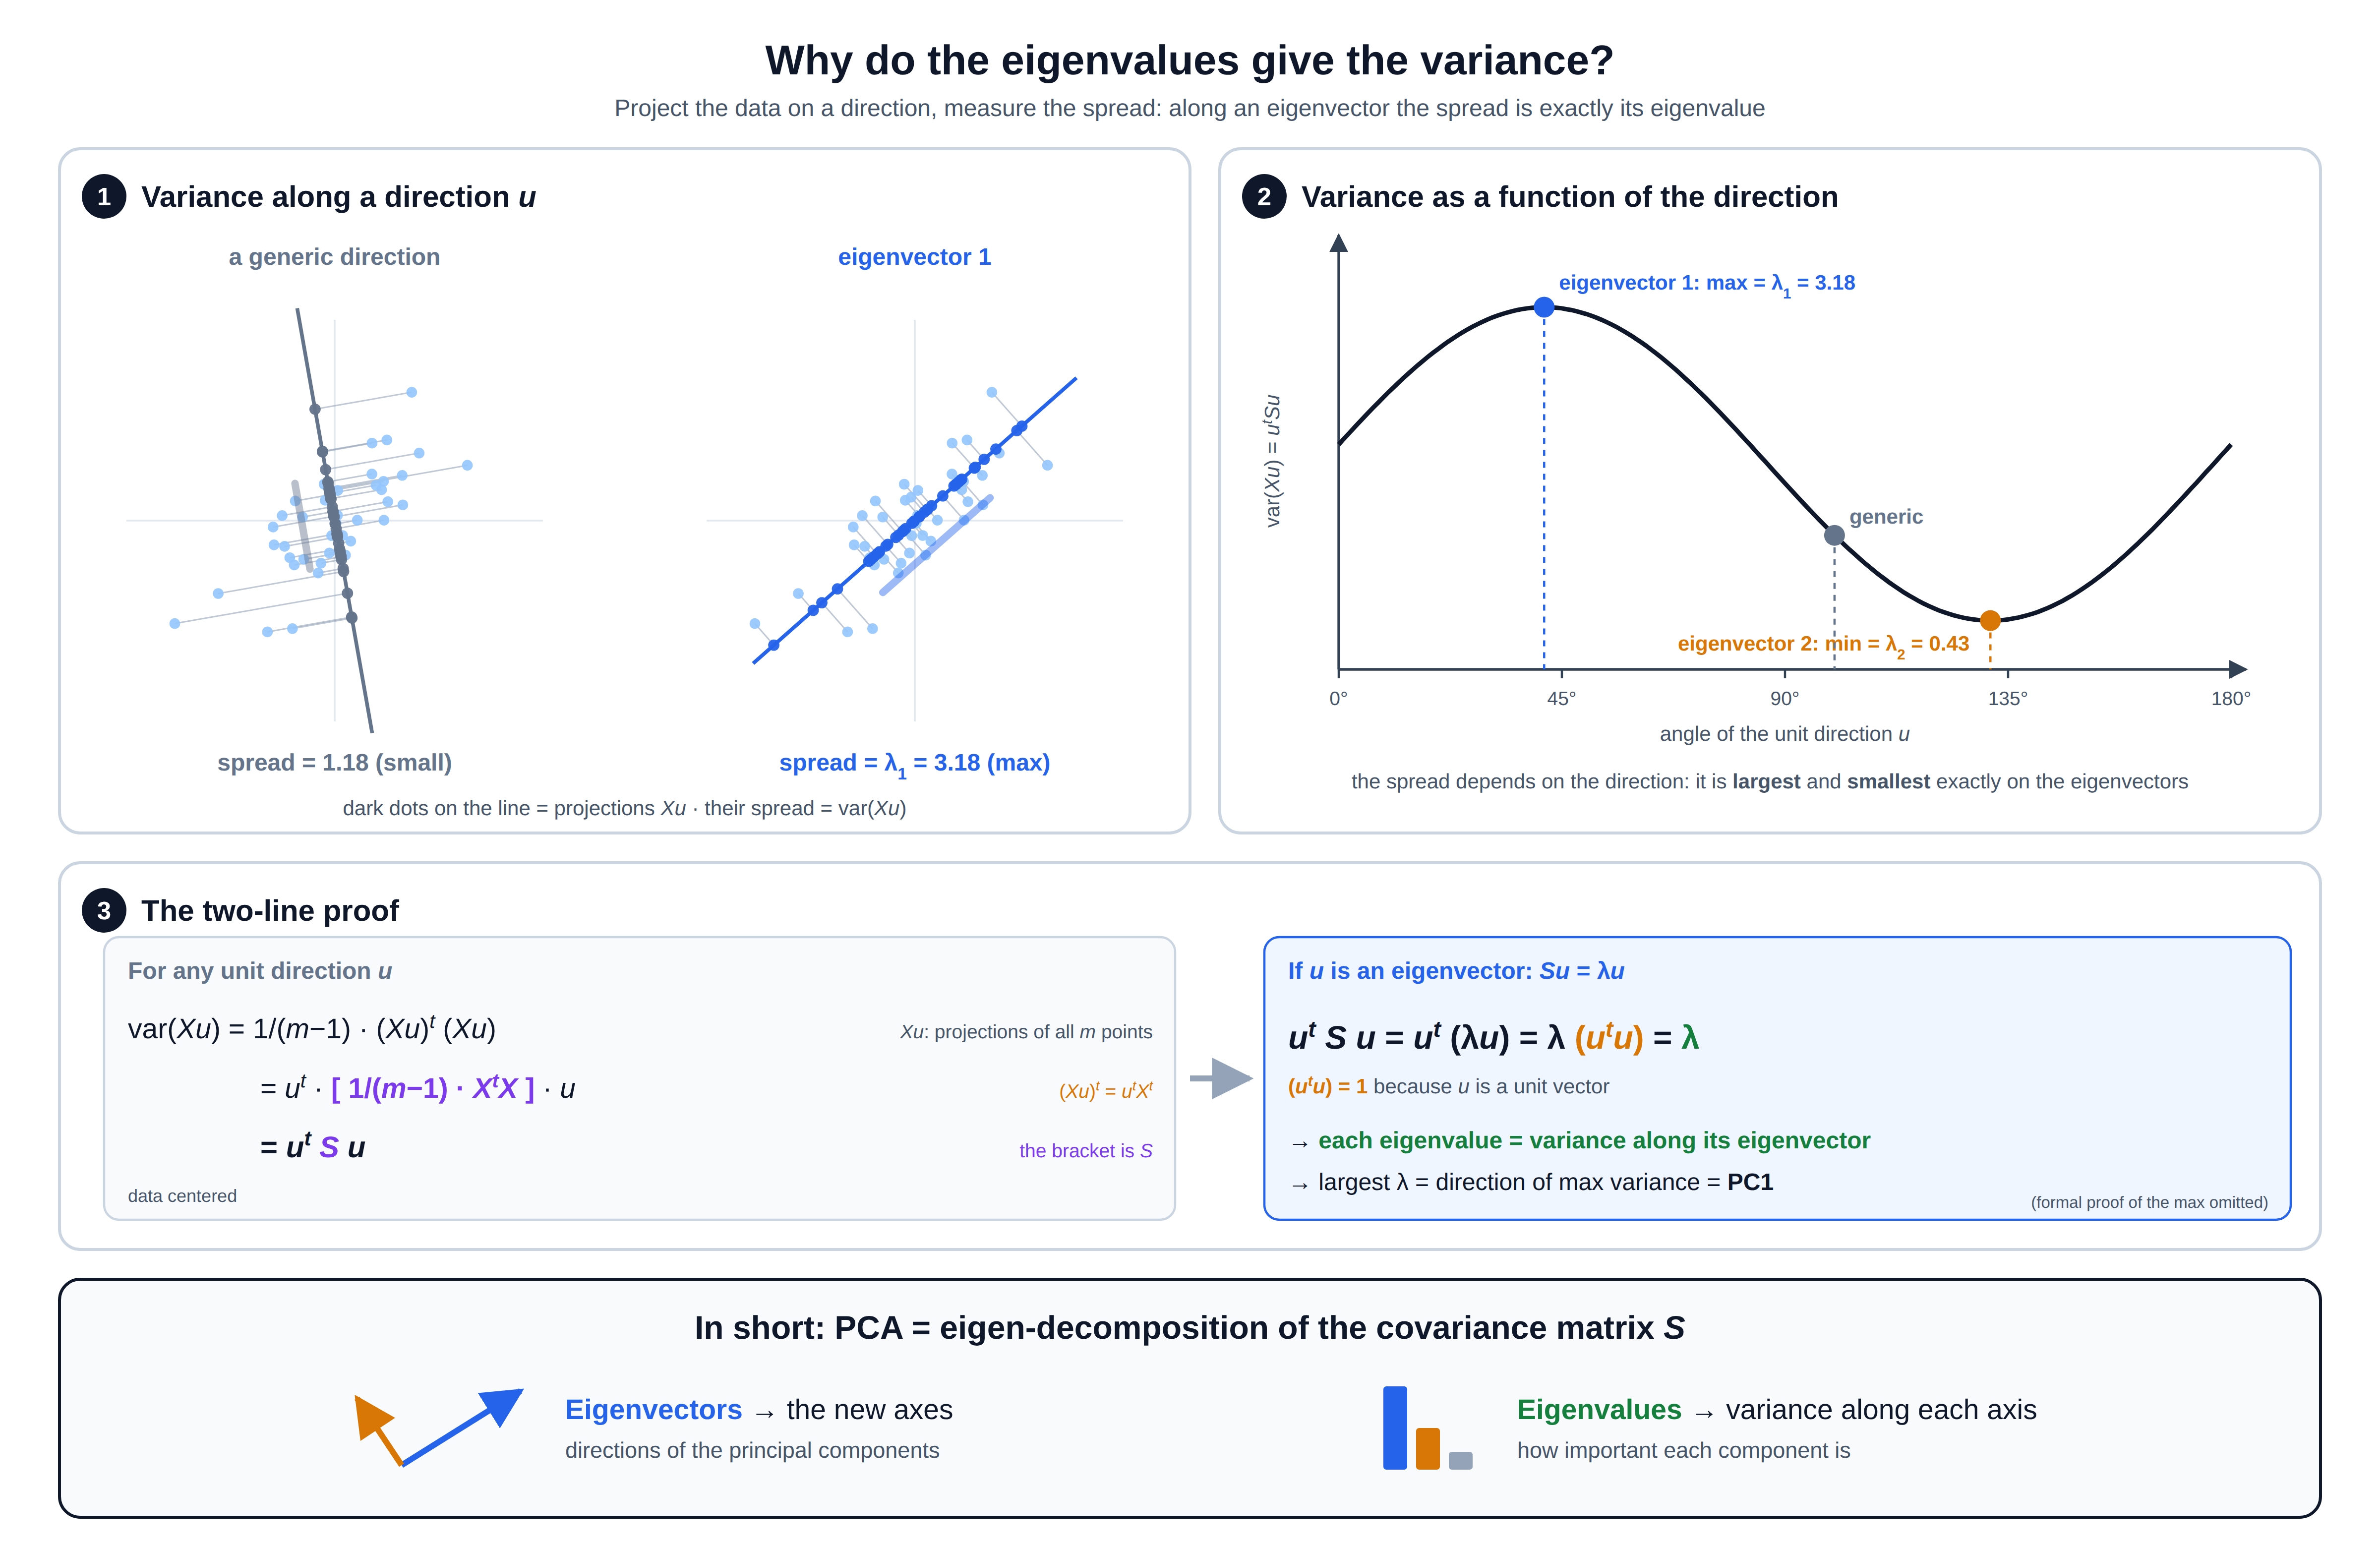
\includegraphics[width=1\textwidth]{images/chapter_4/pca_eigenvalues_variance.png}
    \caption{Each eigenvalue is the variance of the data along its eigenvector}
\end{figure}

\begin{center}
    \fbox{\parbox{0.9\textwidth}{\centering
    \textbf{In short}: PCA $=$ eigen-decomposition of the covariance matrix.\\
    \textbf{Eigenvectors} $\rightarrow$ the new axes (the directions of the principal components).\\
    \textbf{Eigenvalues} $\rightarrow$ the variance along each axis (how important it is).}}
\end{center}

\subsection{Principal Components}
\begin{itemize}
    \item \textbf{PC1} is the eigenvector with the \textbf{largest eigenvalue}: the direction along which the data have the \textbf{greatest variance}.
    \item \textbf{PC2} is the eigenvector with the second largest eigenvalue: the direction of maximum variance \emph{left} in the data, \textbf{orthogonal to PC1}.
    \item The remaining PCs follow in the same way, in order of decreasing eigenvalue.
\end{itemize}

\section{Steps of PCA}
To recap, PCA follows these steps:

\begin{enumerate}
    \item \textbf{Center the data}: subtract the mean of each attribute, $X - \overline{X}$, so that every column has zero mean.
    \item \textbf{Compute the covariance matrix} $S$ ($n \times n$) of the centered data.
    \item \textbf{Find the eigenvectors and eigenvalues} of $S$: each eigenvector is a new axis, and its eigenvalue $\lambda$ is the variance along it.
    \item \textbf{Sort} the eigenvectors by decreasing $\lambda$, from the most to the least important direction.
    \item \textbf{Select} the eigenvectors of the top $p$ eigenvalues and use them as rows of $P$ ($p \times n$).
    \item \textbf{Project} the data: $X' = XP^t$, an $m \times p$ matrix, i.e.\ the same $m$ points described by only $p$ features.
\end{enumerate}

Since each eigenvalue is a variance, the percentage of the total variance explained by component $i$ is its share of the sum:

\begin{figure}[h]
    \centering
    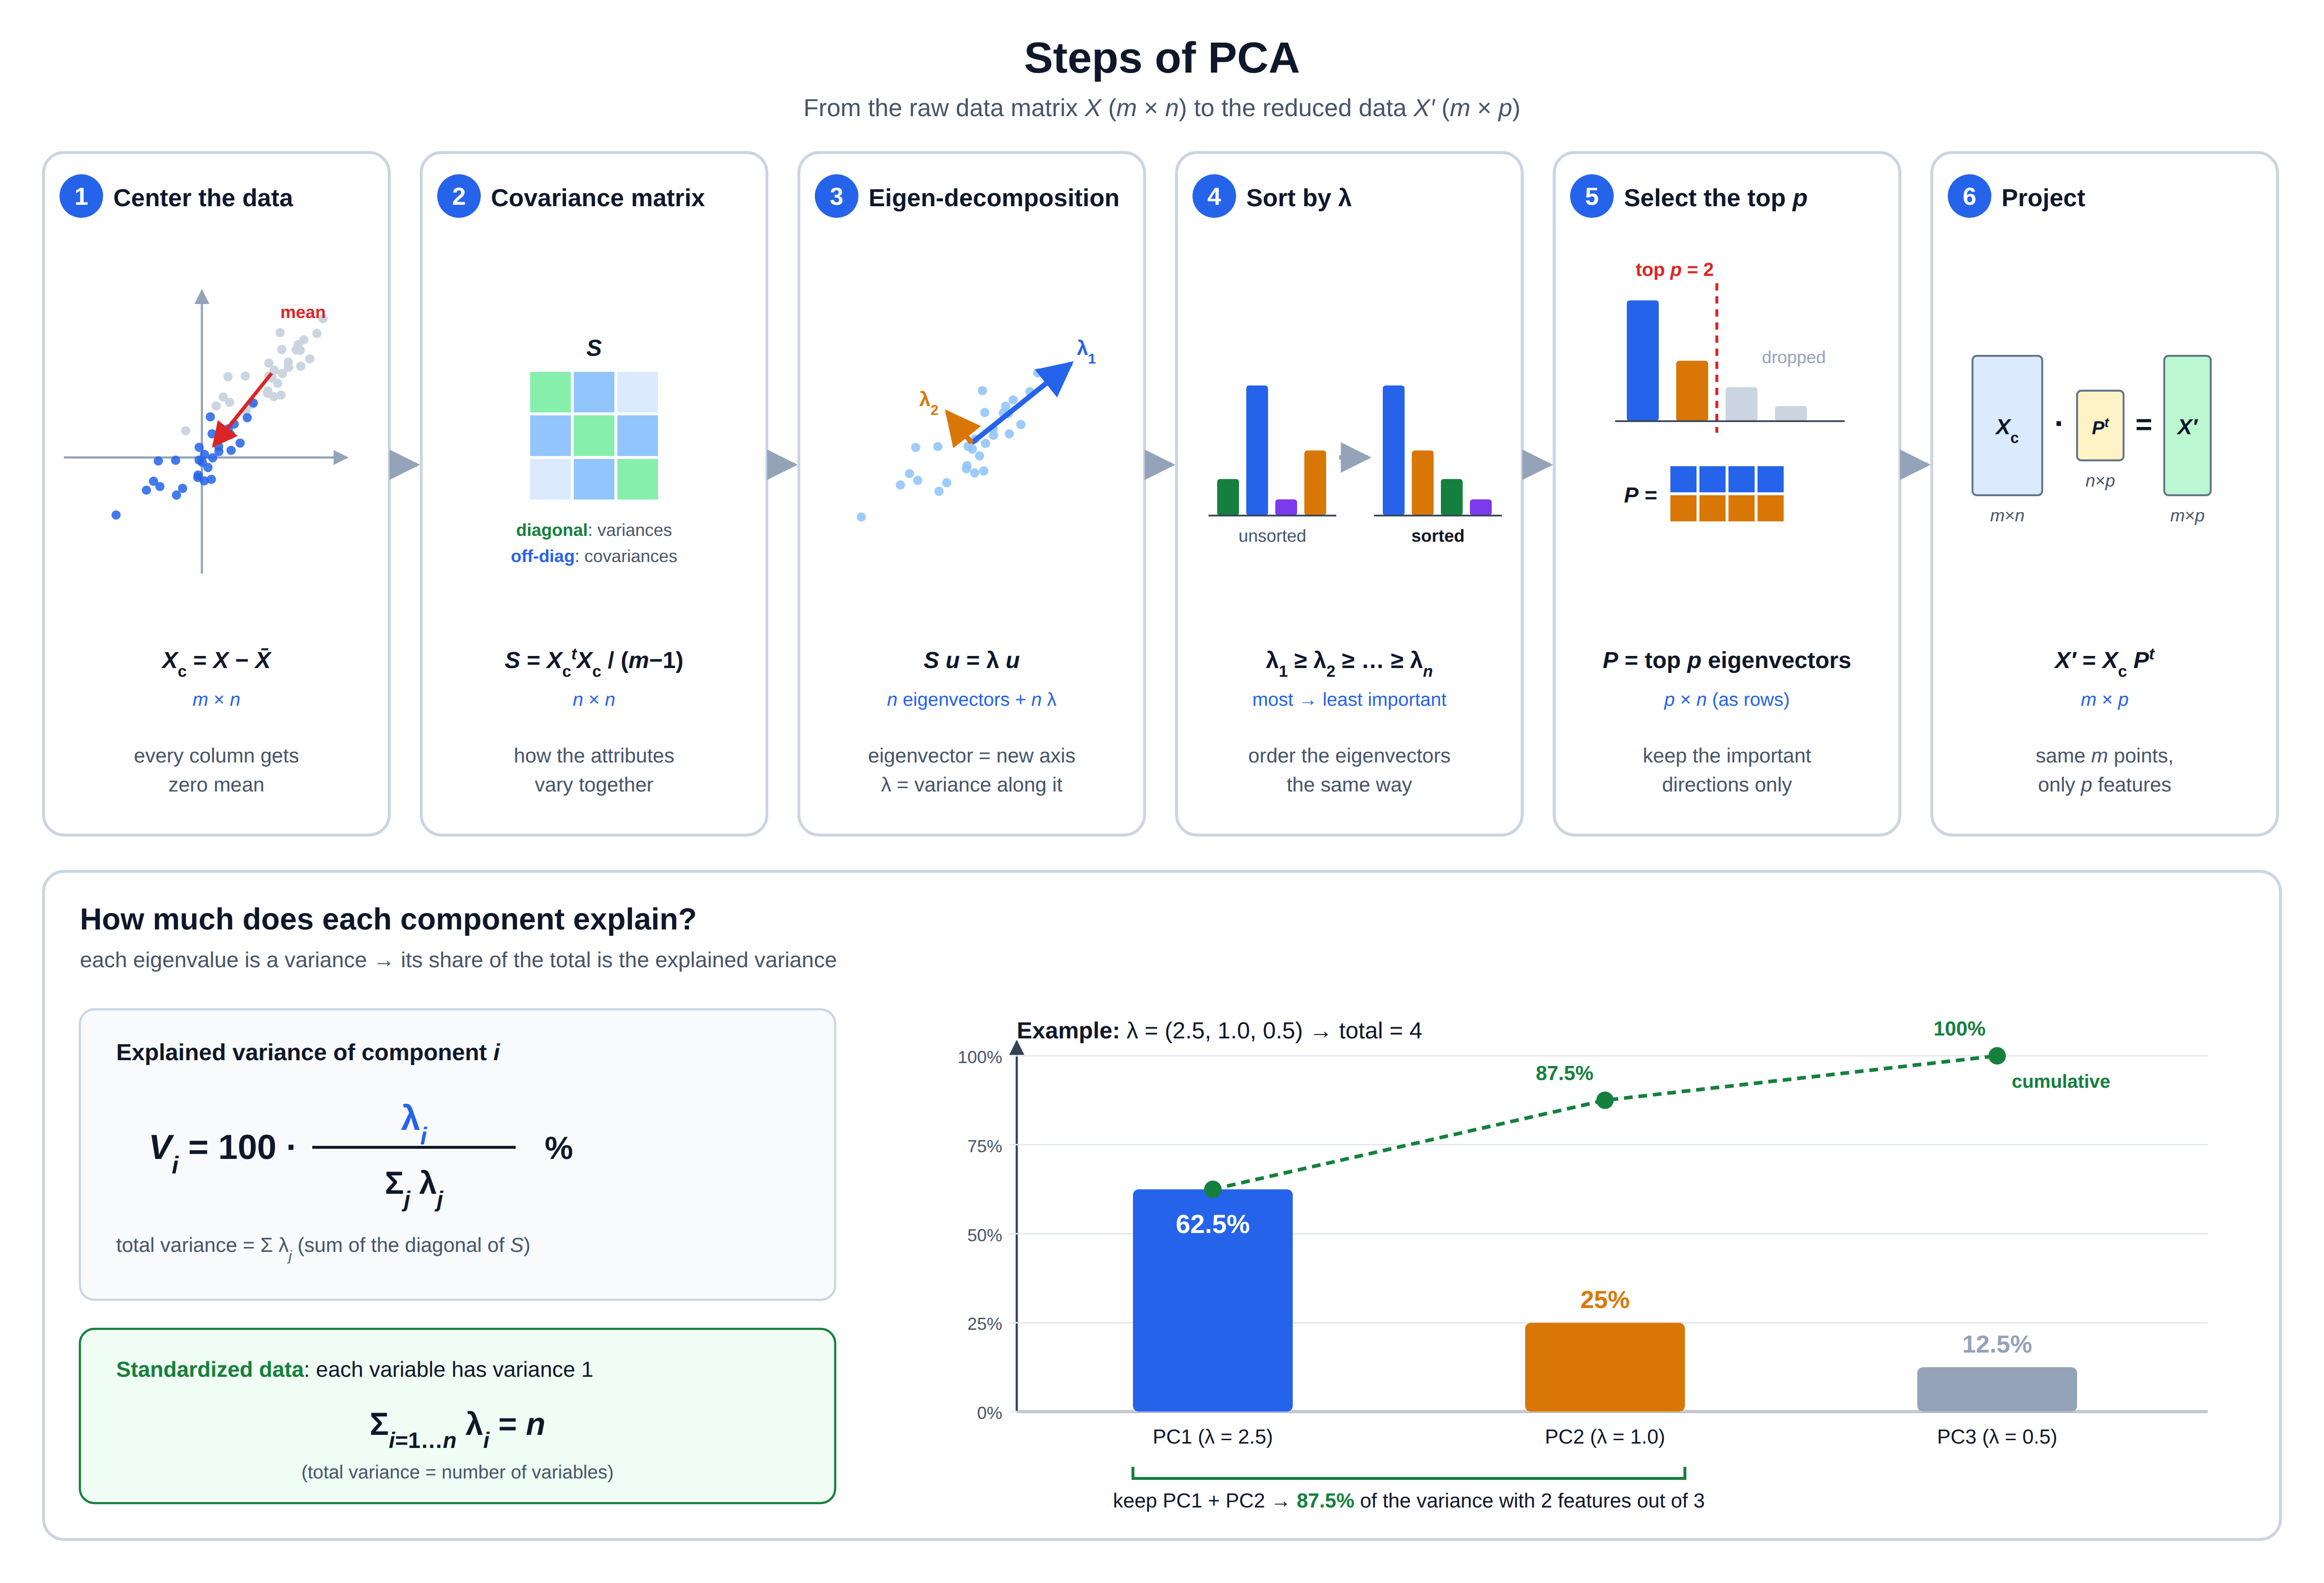
\includegraphics[width=1\textwidth]{images/chapter_4/pca_steps.png}
    \caption{The six steps of PCA and the explained variance}
\end{figure}

\begin{figure}[h!]
    \centering
    \begin{minipage}{0.7\textwidth}
    \[
        V_i = 100 \, \frac{\lambda_i}{\sum_{j=1}^{n} \lambda_j}
    \]
    \[
        \sum_{i=1}^{n} \lambda_i = n \quad \text{(for standardized data: each variable has variance 1)}
    \]
    \emph{Example}: with $\lambda = (2.5,\ 1.0,\ 0.5)$ the total is 4, so PC1 explains $62.5\%$, PC2 $25\%$ and PC3 $12.5\%$. Keeping only PC1 and PC2 preserves $87.5\%$ of the variance.
    \end{minipage}
    \caption{Eigenvalues and Variance}
\end{figure}

\subsection{Properties of Principal Components}
The resulting Principal Components:

\begin{itemize}
    \item are \textbf{linear combinations} of the original variables;
    \item are \textbf{uncorrelated} with each other;
    \item capture \textbf{as much of the original variance as possible}.
\end{itemize}

PCA is \textbf{sensitive to scale}. If one variable is measured in meters and another in millimeters, the second has a much larger variance only because of its unit, and it would dominate PC1. PCA should therefore be applied to variables on approximately the same scale. It is good practice to \textbf{standardize} the data first (zero mean and unit variance for each variable), so that all variables carry the same weight.

\textbf{Choice of $p$} (how many principal components to keep):

\begin{itemize}
    \item \textbf{Kaiser criterion}: keep the PCs with eigenvalue $> 1$. With standardized data each original variable has variance 1, so a PC with $\lambda > 1$ explains more than a single original variable.
    \item \textbf{Proportion of variance explained}: keep PCs until the cumulative explained variance exceeds a threshold (e.g.\ 80--90\%).
    \item \textbf{Elbow method}: plot the eigenvalues in decreasing order (\emph{scree plot}); the point where the curve bends and flattens (the ``elbow'') indicates how many components to retain.
\end{itemize}

\section{Non-linear Dimensionality Reduction}
PCA finds only \emph{linear} axes, so in some cases it does not perform well. For example, circularly-shaped data require \textbf{non-linear axes}.

\begin{figure}[h]
    \centering
    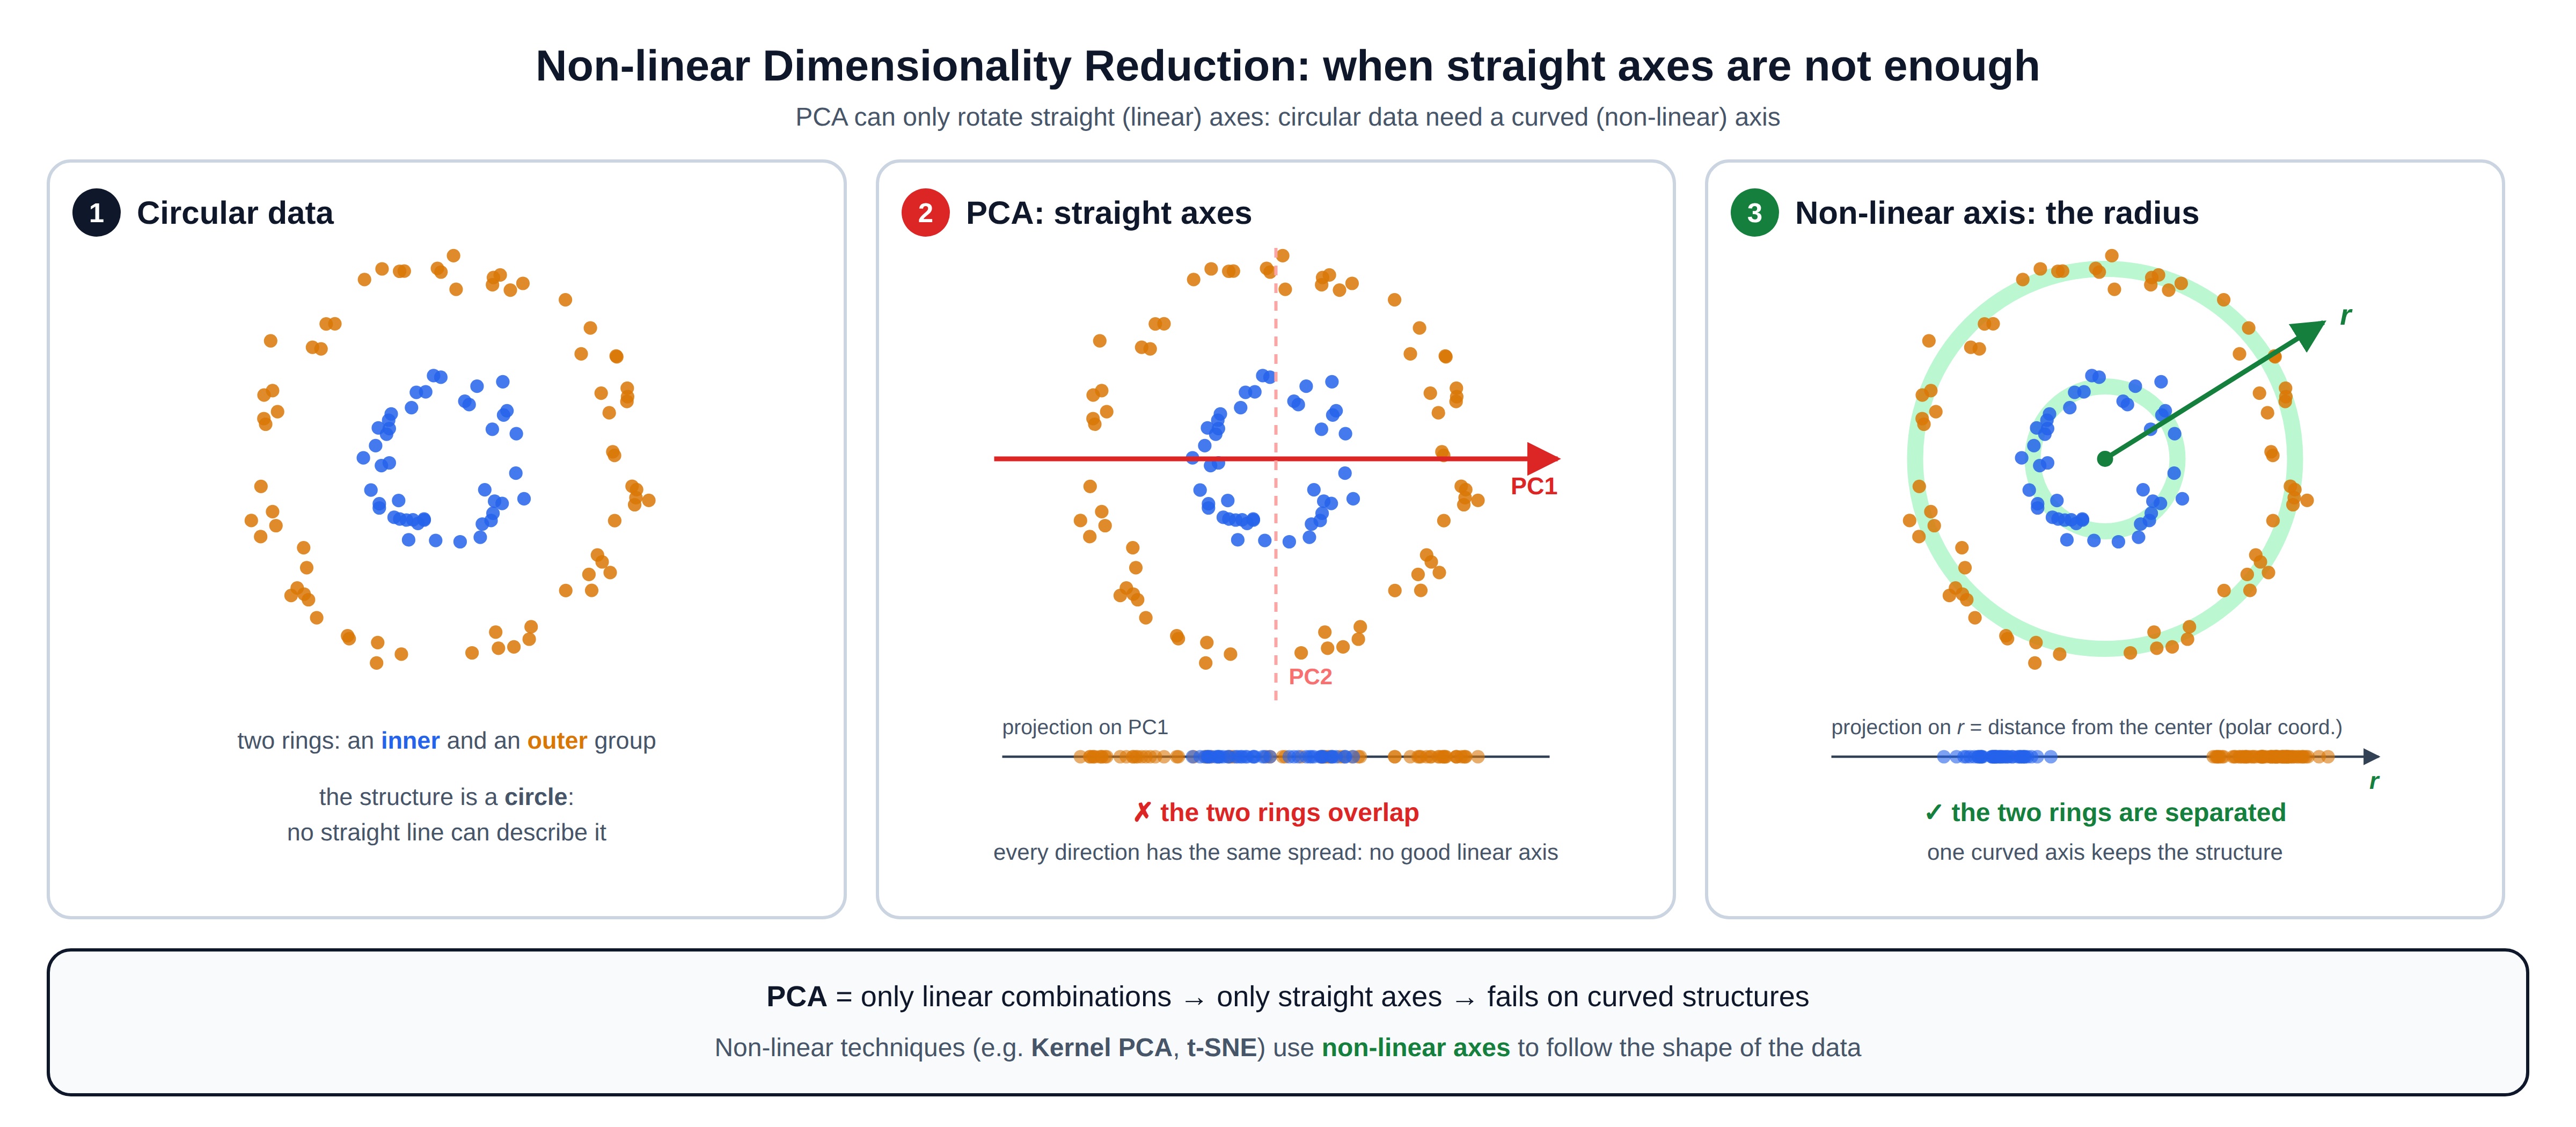
\includegraphics[width=1\textwidth]{images/chapter_4/nonlinear_dr_intro.png}
    \caption{Circular data: PCA's straight axes fail, a non-linear axis (the radius) works}
\end{figure}

\subsection{Kernel PCA}
Kernel PCA extends PCA. Instead of using the points $x$ directly, it maps them to a different feature space $f(x)$, for instance polar coordinates instead of Cartesian ones. PCA is then performed in this new space, giving components that are \textbf{non-linear with respect to the original space}.

\begin{figure}[h!]
    \centering
    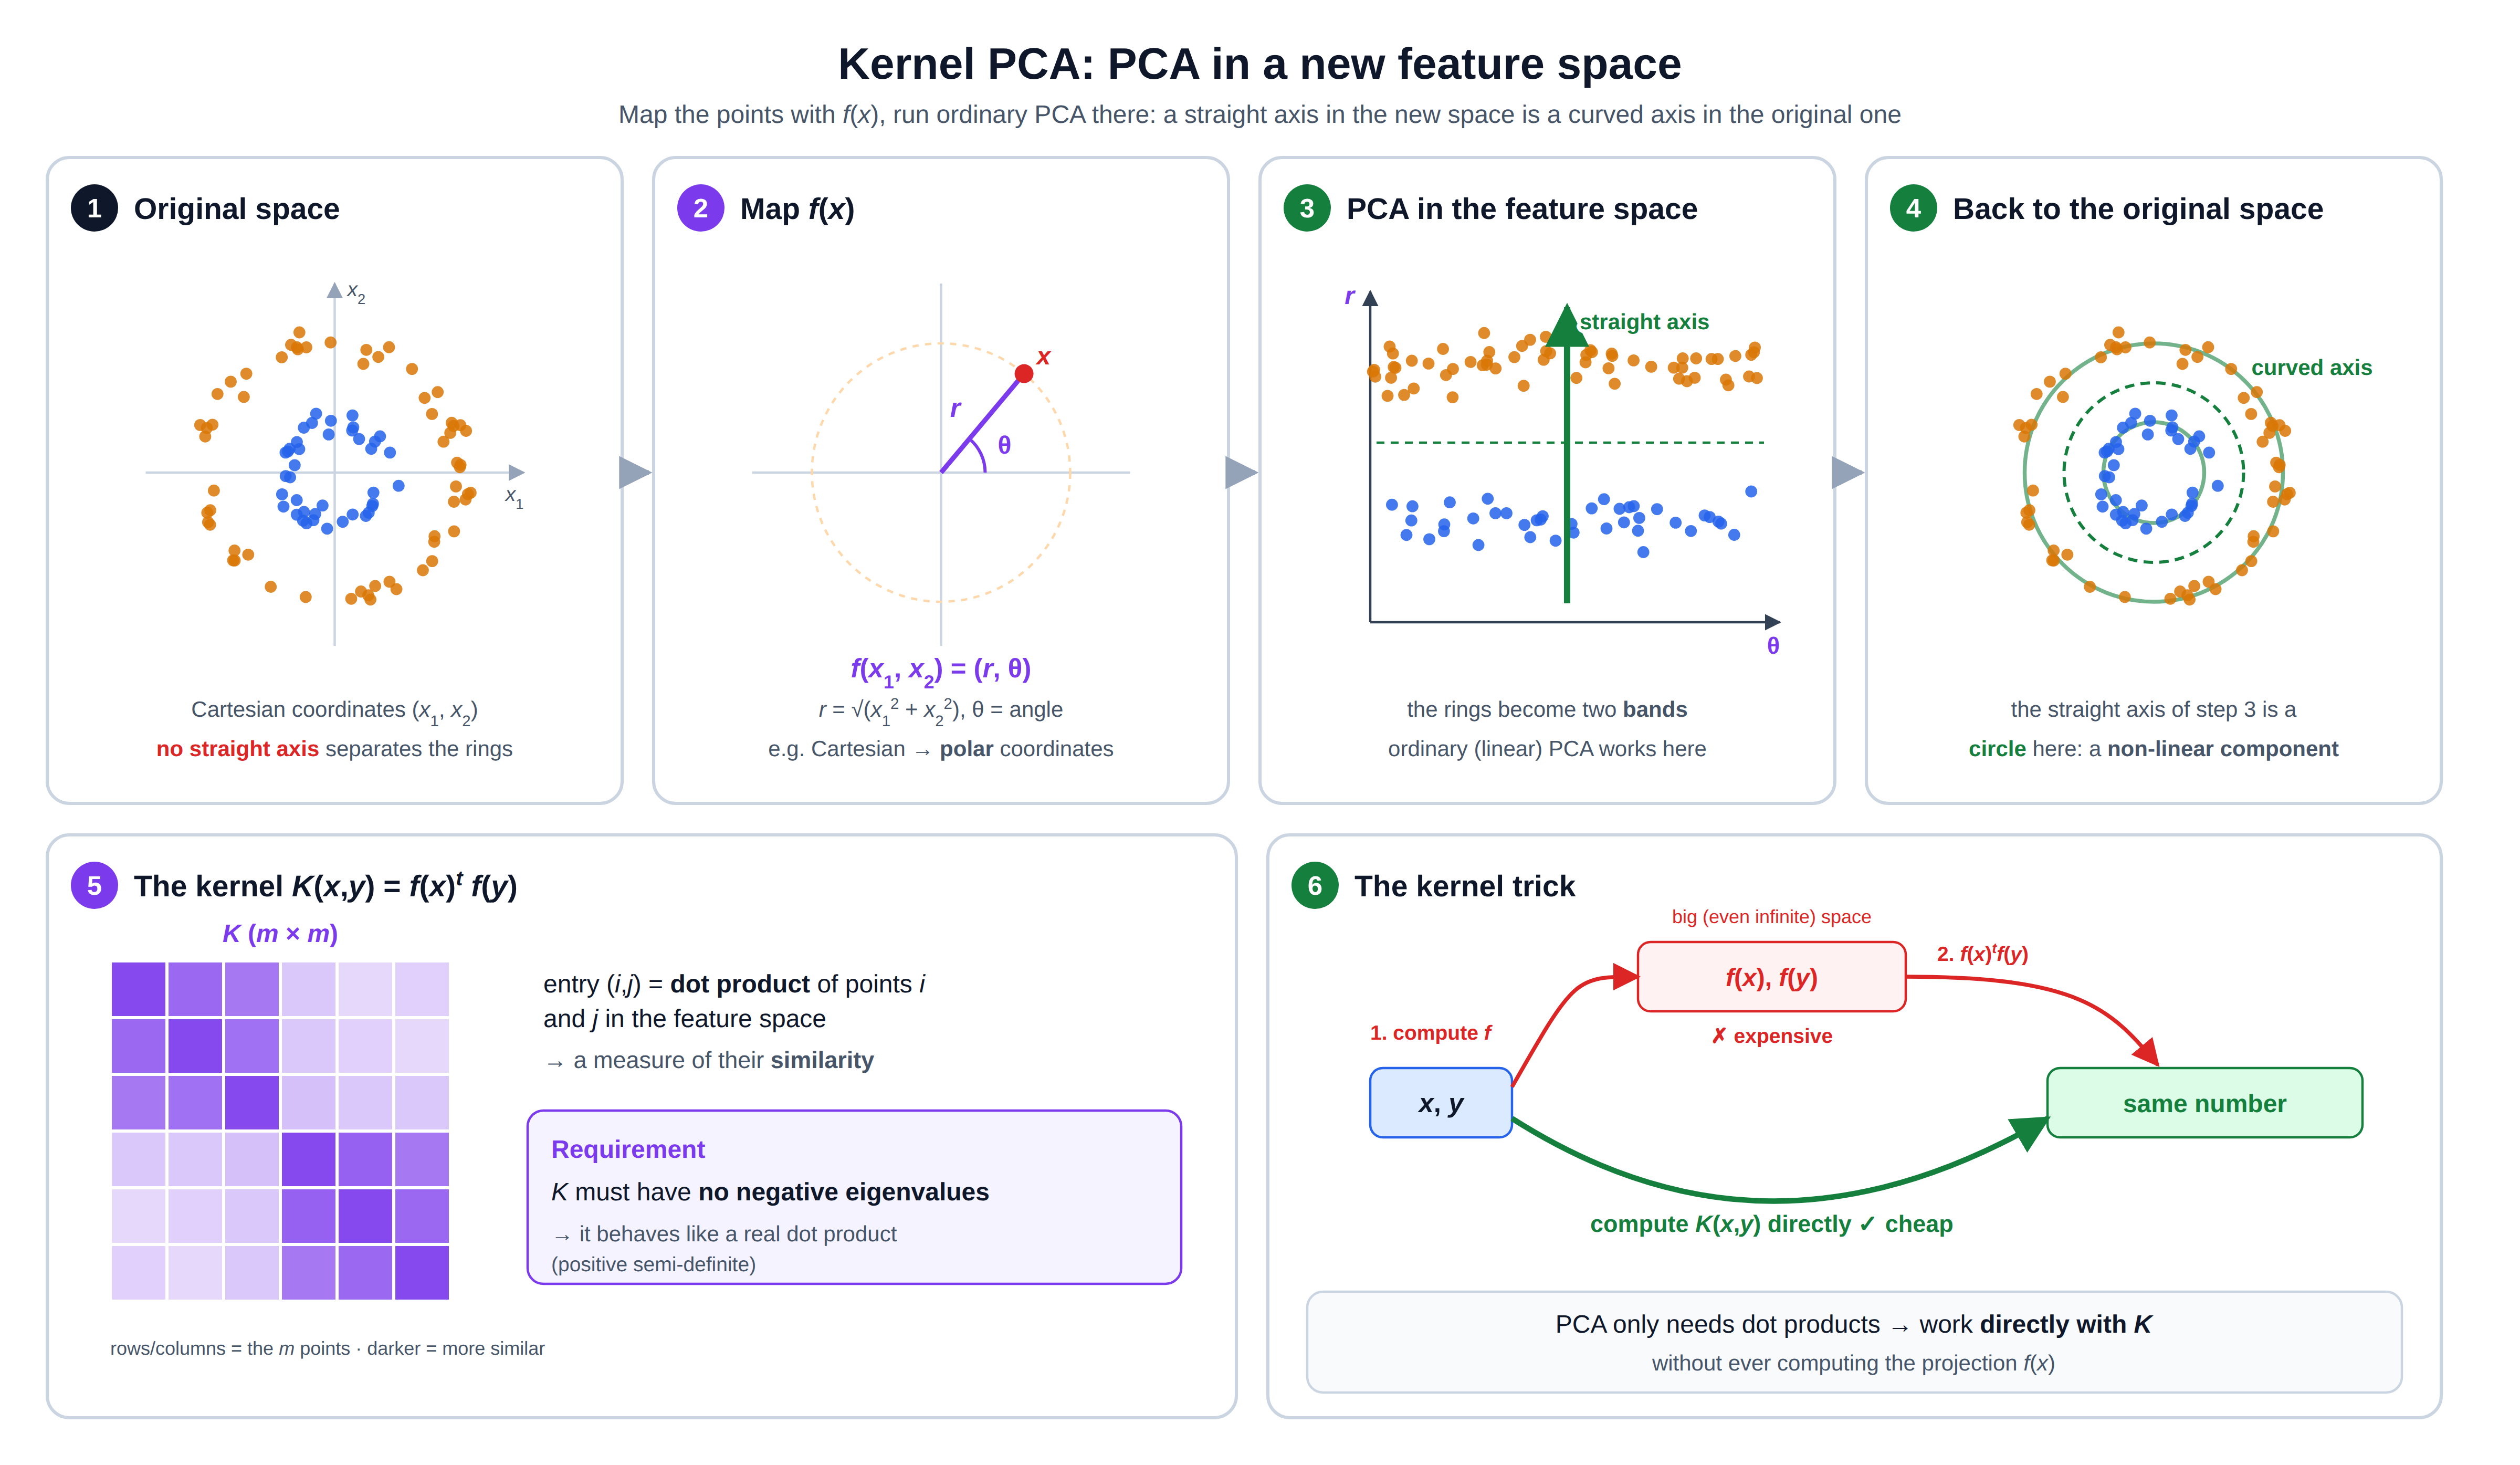
\includegraphics[width=0.5\textwidth]{images/chapter_4/kernel_pca.png}
    \caption{Kernel PCA: PCA in a feature space and the kernel trick}
\end{figure}

The map $f$ must be such that the kernel $K(x, y) = f(x)^t f(y)$ has \textbf{no negative eigenvalues}. In practice one can work \textbf{directly with the kernel matrix $K$}, without explicitly computing the projection $f(x)$ (the \emph{kernel trick}).


\subsection{t-SNE}
t-SNE is a non-linear dimensionality reduction technique designed to \textbf{embed high-dimensional data for visualization}. Similar objects are mapped to nearby points and dissimilar objects to distant points, with high probability.

\begin{figure}[h!]
    \centering
    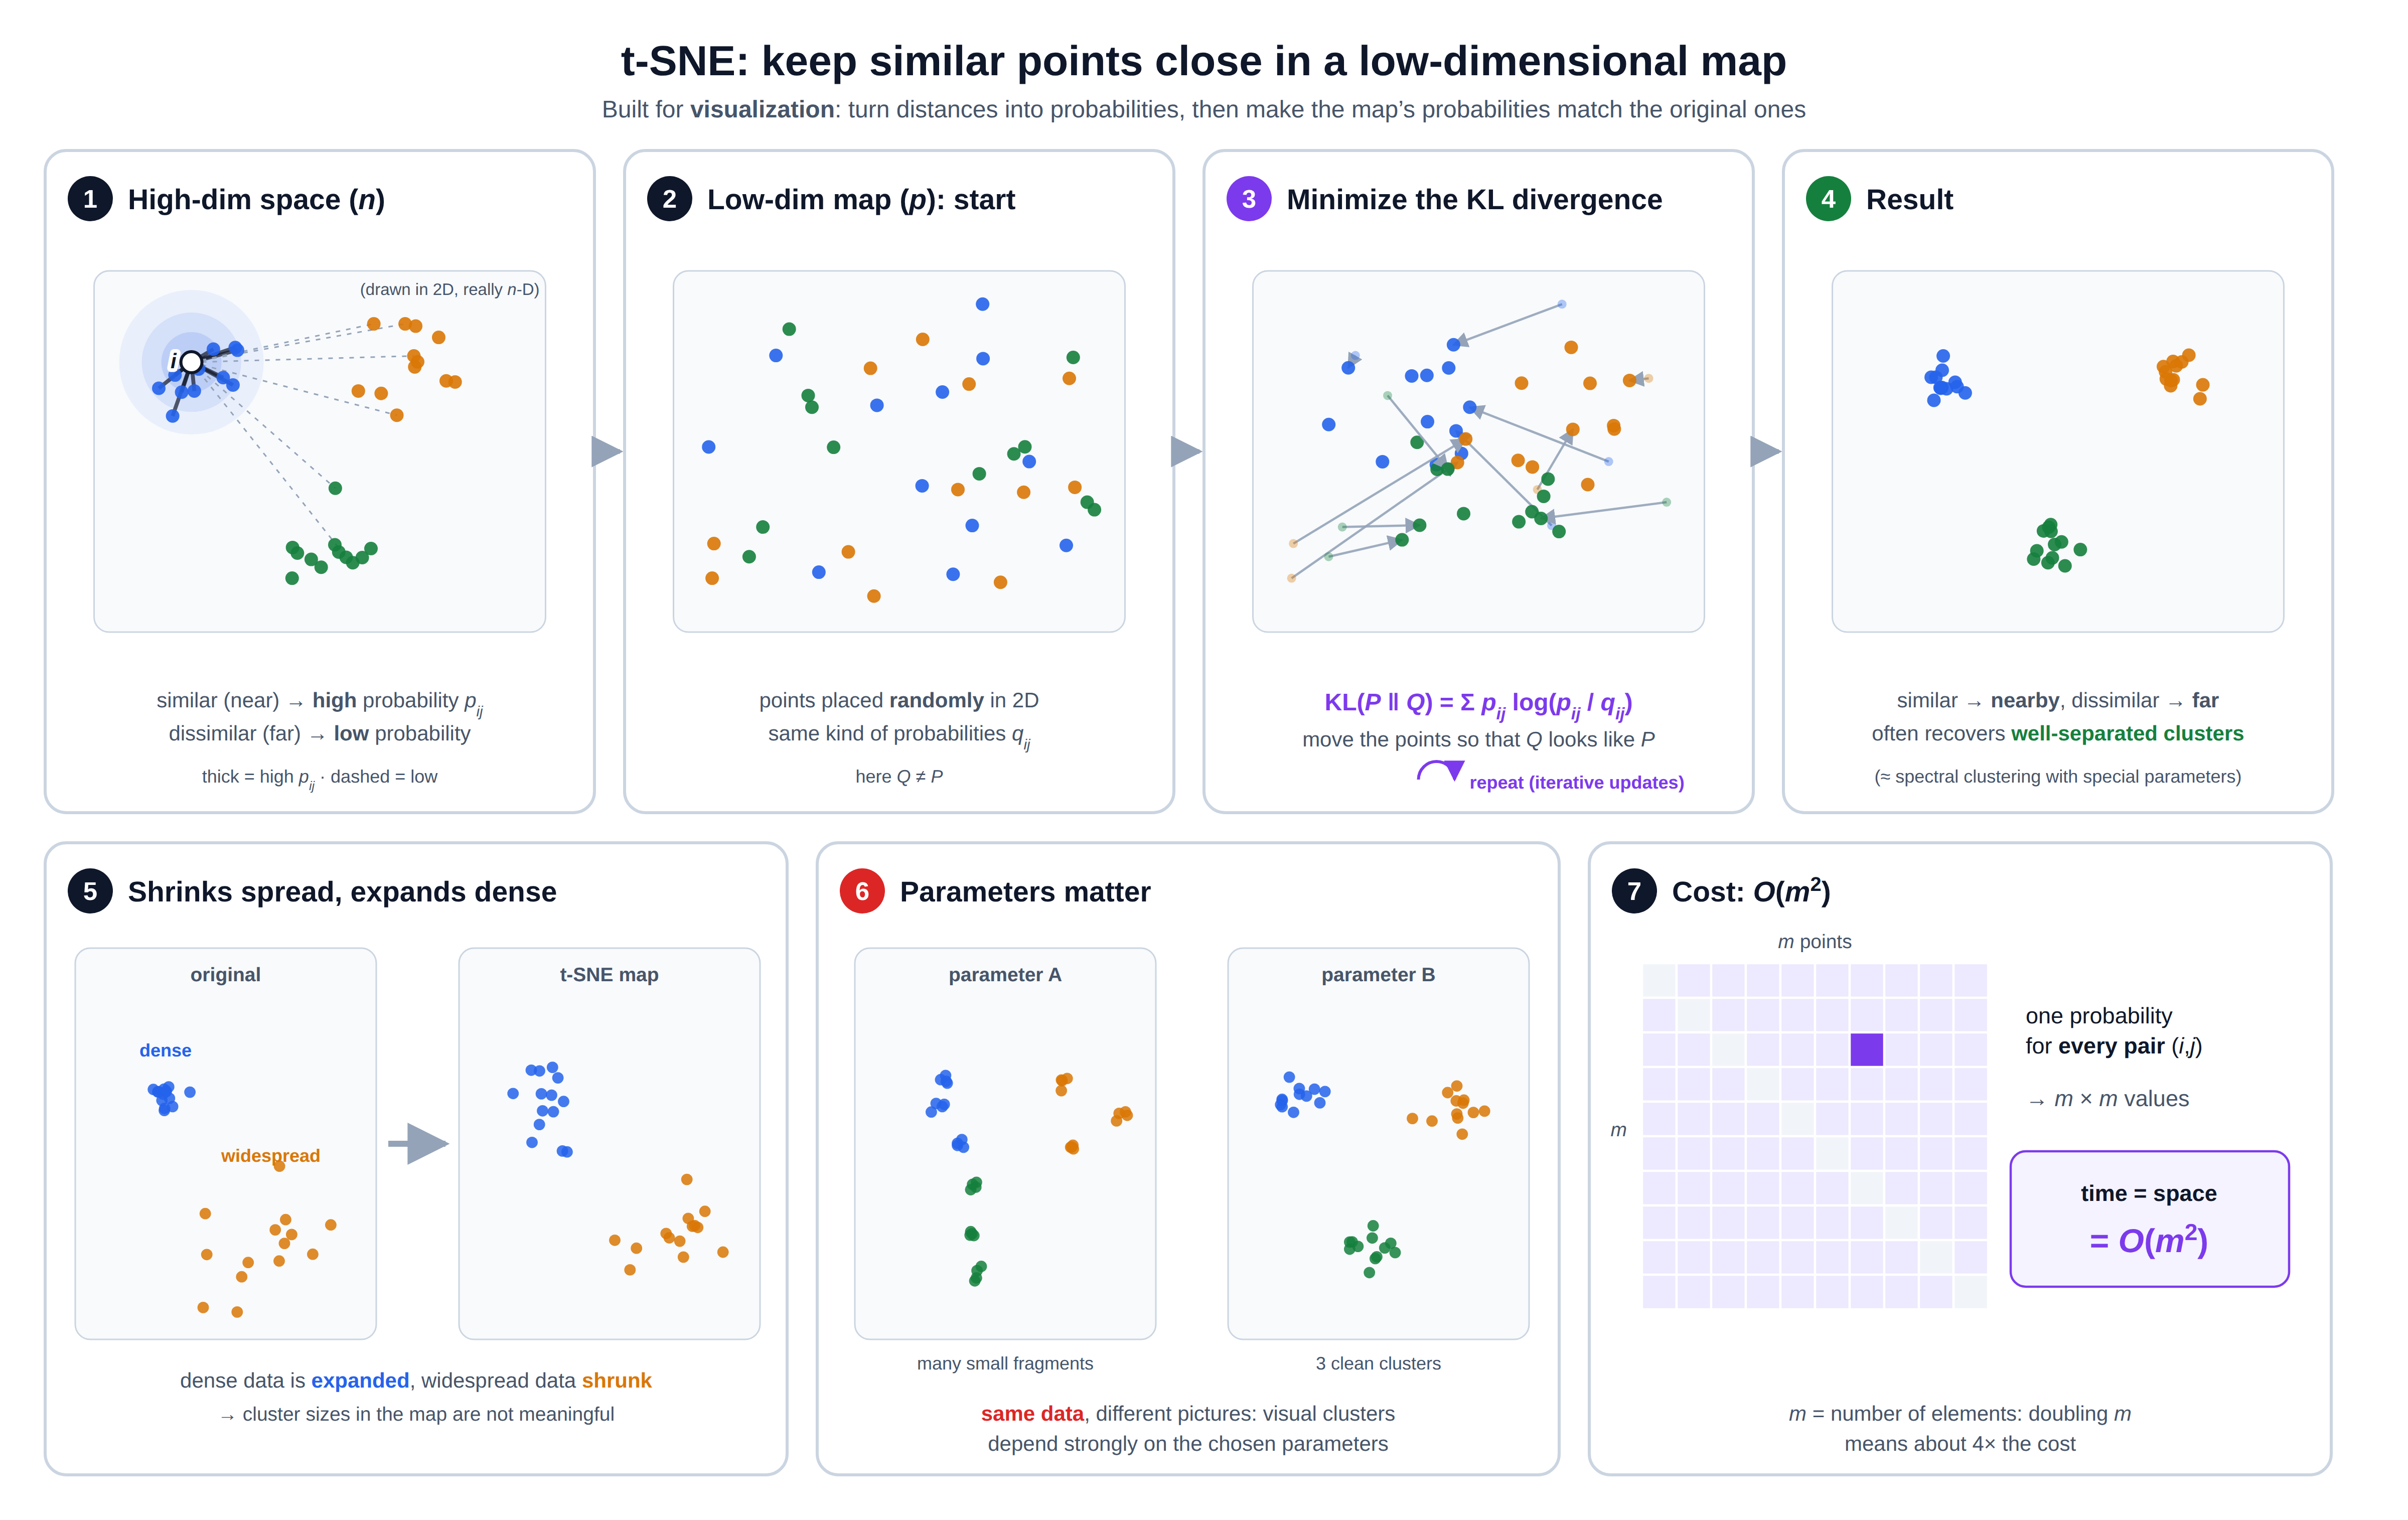
\includegraphics[width=0.5\textwidth]{images/chapter_4/tsne.png}
    \caption{t-SNE: from pairwise probabilities to a low-dimensional map}
\end{figure}

t-SNE works in 2 stages:

\begin{enumerate}
    \item In the \textbf{high-dimensional space} ($n$), build a probability distribution over pairs of objects. Similar objects get a high probability and dissimilar ones a low probability.
    \item In the \textbf{low-dimensional map} ($p$), define a similar probability distribution over the corresponding points.
\end{enumerate}

The low-dimensional map is then \textbf{iteratively updated} to minimize the \textbf{Kullback--Leibler divergence} between the two distributions. The goal is to make the $n$-space and $p$-space distributions as similar as possible.

Behaviour of t-SNE:
\begin{itemize}
    \item It \textbf{shrinks widespread data} and \textbf{expands densely packed data}.
    \item It often recovers \textbf{well-separated clusters}; with special parameter choices, it approximates a simple form of spectral clustering.
    \item The visual clusters can be \textbf{strongly influenced by the chosen parameters}.
\end{itemize}

Both its time and space complexity, with $m$ the number of elements, are:
\[
    \text{Complexity}_{\text{t-SNE}} = O(m^2)
\]

\subsection{PCA vs t-SNE}

\begin{itemize}
    \item \textbf{Distances}: t-SNE preserves \textbf{small pairwise distances} (local structure). PCA preserves \textbf{large pairwise distances} (global structure), in order to maximize the variance.
    \item \textbf{What is preserved}: PCA preserves the \textbf{variance} of the data. t-SNE preserves the \textbf{relationships between data points} in the lower-dimensional space, which makes it well suited to visualizing complex high-dimensional data.
\end{itemize}

\begin{figure}[h!]
    \centering
    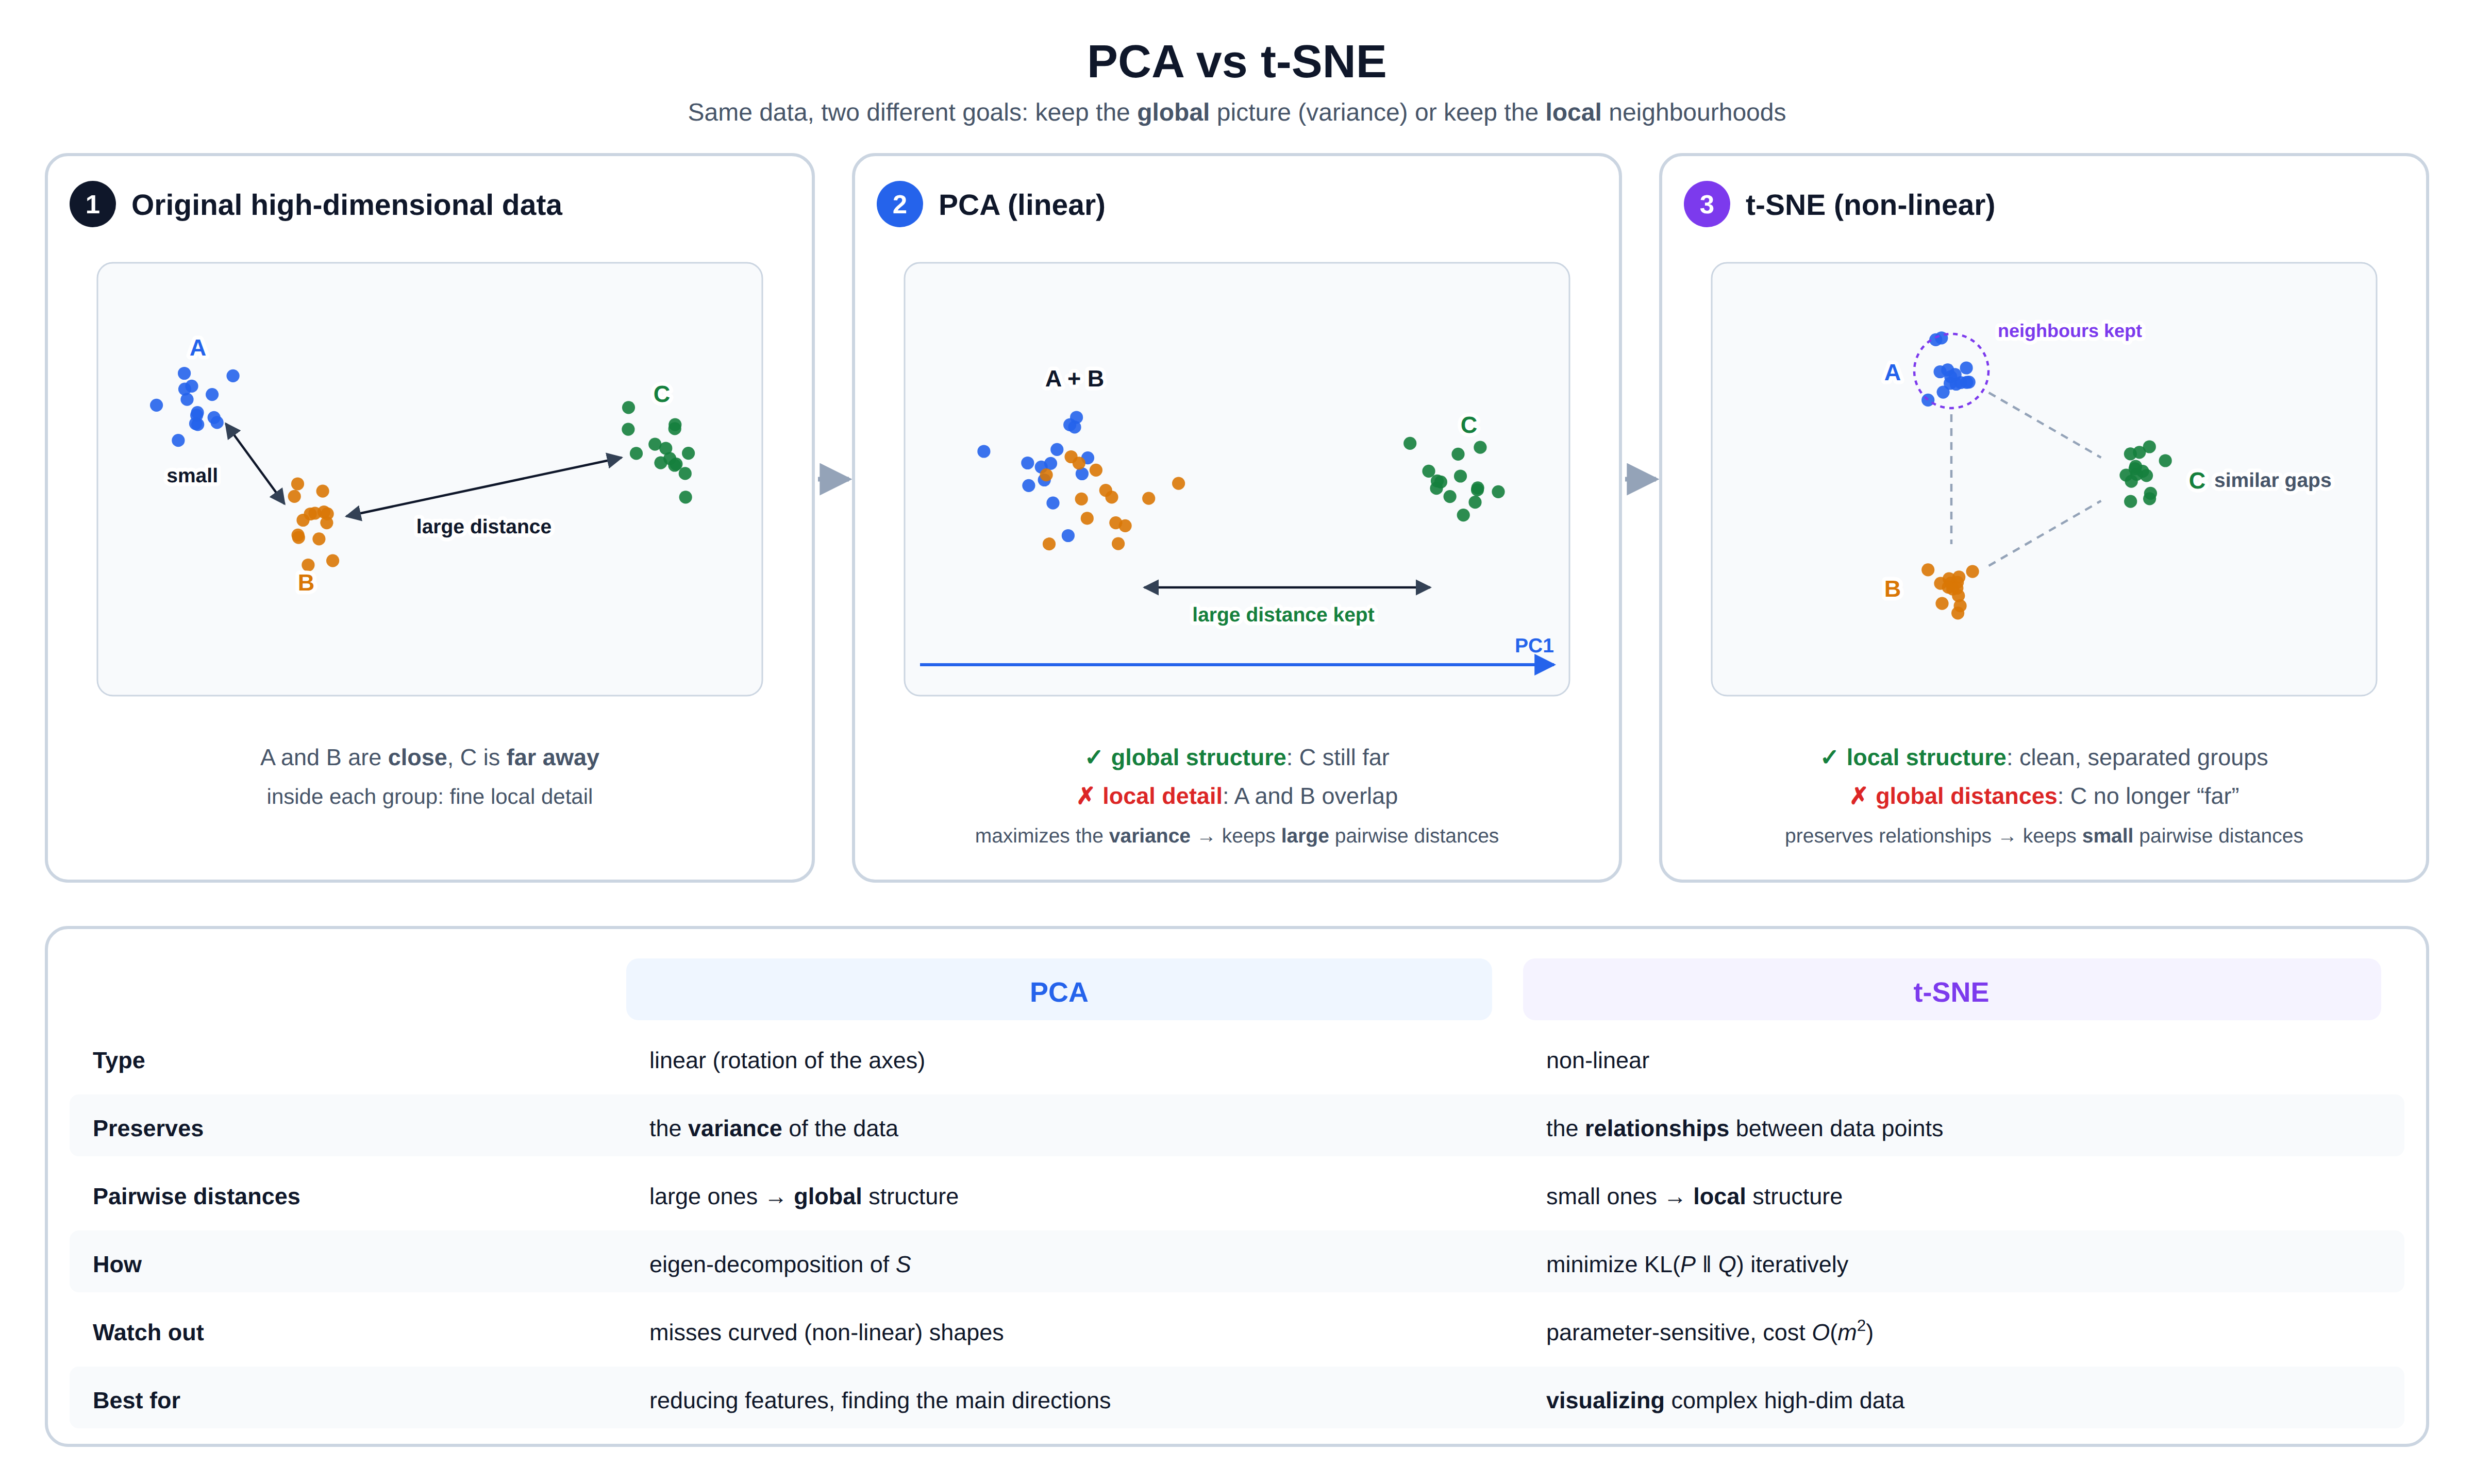
\includegraphics[width=1\textwidth]{images/chapter_4/pca_vs_tsne.png}
    \caption{PCA vs t-SNE: global vs local structure}
\end{figure}

\begin{figure}[h!]
    \centering
    \begin{minipage}{0.75\textwidth}
    \begin{itemize}
        \item Consider the following 5 samples with 4 features. Compute the principal components and their explained variance.
        \item For eigenvalues and eigenvectors, you can use Python (note: \texttt{eig} returns the eigenvectors as \emph{columns}):\\
        \texttt{from numpy.linalg import eig}\\
        \texttt{eigenvalues, eigenvectors = eig(A)}
    \end{itemize}

    \vspace{0.3cm}
    \centering
    \begin{tabular}{cccc}
        \toprule
        f1 & f2 & f3 & f4 \\
        \midrule
        1 & 2 & 3 & 4 \\
        5 & 5 & 6 & 7 \\
        1 & 4 & 2 & 3 \\
        5 & 3 & 2 & 1 \\
        8 & 1 & 2 & 2 \\
        \bottomrule
    \end{tabular}
    \end{minipage}
    \caption{Self-Assessment Quiz Chapter 4}
\end{figure}


\section{A prova di coglione}

\paragraph*{Il problema e l'idea.}
Quando i dati hanno molte dimensioni diventano difficili da visualizzare e da analizzare: è la \textbf{maledizione della dimensionalità}. La \textbf{Dimensionality Reduction} risolve il problema \emph{cambiando punto di vista}. I dati vengono descritti con \textbf{meno feature} ($p < n$), conservando l'informazione importante ed eliminando ridondanza e rumore. Lo schema è sempre lo stesso:
\begin{itemize}
    \item una funzione $h$ \textbf{comprime} il dato da $n$ a $p$ feature;
    \item una funzione $g$ lo \textbf{ricostruisce}, ottenendo $x' \approx x$;
    \item l'obiettivo è comprimere il più possibile con il minimo errore di ricostruzione.
\end{itemize}
I vantaggi sono modelli più leggeri e veloci, meno overfitting, meno rumore e dati visualizzabili.

\paragraph*{PCA: l'intuizione.}
La PCA è una \textbf{rotazione degli assi}. Si cerca un nuovo sistema di riferimento ortogonale in cui:
\begin{itemize}
    \item il \textbf{primo asse} segue la direzione di \textbf{massima varianza} dei dati;
    \item il secondo segue la massima varianza residua, ortogonale al primo, e così via.
\end{itemize}
Le nuove variabili, le \textbf{componenti principali}, sono combinazioni lineari di quelle originali e sono \textbf{scorrelate} tra loro. Se le variabili originali sono ridondanti (correlate), poche componenti bastano a spiegare quasi tutta la varianza. Massimizzare la varianza proiettata equivale a minimizzare l'errore di proiezione, cioè di ricostruzione: sono due facce dello stesso problema.

\paragraph*{PCA: la matematica in una riga.}
Tutto ruota attorno alla \textbf{matrice di covarianza} $S$ dei dati centrati:
\begin{itemize}
    \item gli \textbf{autovettori} di $S$ sono le nuove direzioni (gli assi principali);
    \item gli \textbf{autovalori} sono le varianze lungo quelle direzioni.
\end{itemize}
Usando gli autovettori come righe di $P$, la proiezione $X' = XP^t$ ha covarianza \textbf{diagonale}: le nuove feature non sono correlate. La quota di varianza spiegata dalla componente $i$ è
\[
    V_i = 100\,\frac{\lambda_i}{\sum_j \lambda_j}.
\]

\paragraph*{PCA in pratica.}
\begin{enumerate}
    \item Centrare (meglio ancora, \textbf{standardizzare}) i dati.
    \item Calcolare la matrice di covarianza.
    \item Calcolarne autovalori e autovettori.
    \item Ordinarli per autovalore decrescente.
    \item Tenere i primi $p$ autovettori.
    \item Proiettare i dati su di essi.
\end{enumerate}

Per scegliere $p$ ci sono tre criteri:
\begin{itemize}
    \item \textbf{Kaiser}: tenere le componenti con autovalore $> 1$;
    \item \textbf{soglia di varianza cumulata}: tenere componenti finché si supera, ad esempio, l'80--90\%;
    \item \textbf{metodo del gomito}: fermarsi dove la curva degli autovalori piega.
\end{itemize}

La standardizzazione è importante perché la PCA è sensibile alla scala: una variabile con valori grandi dominerebbe la varianza.

\paragraph*{Quando la PCA non basta.}
La PCA trova solo \textbf{assi lineari}. Se la struttura dei dati è non lineare, ad esempio dati disposti a cerchio, servono altri metodi:
\begin{itemize}
    \item \textbf{Kernel PCA}: i dati vengono mappati in un nuovo spazio $f(x)$ dove la struttura diventa lineare, e lì si applica la PCA. Grazie al kernel $K(x,y) = f(x)^t f(y)$ non serve calcolare esplicitamente $f$. Il risultato sono componenti non lineari nello spazio originale.
    \item \textbf{t-SNE}: è pensato per la \textbf{visualizzazione}. Costruisce una distribuzione di probabilità di ``vicinanza'' tra le coppie di punti nello spazio originale e una analoga nella mappa a bassa dimensione. Poi modifica la mappa finché le due distribuzioni sono il più simili possibile (minimizzando la divergenza di Kullback--Leibler). Punti simili finiscono vicini e punti diversi lontani. Fa emergere bene i cluster, ma il risultato dipende molto dai parametri e il costo è $O(m^2)$.
\end{itemize}

\paragraph*{PCA vs t-SNE a colpo d'occhio.}
\begin{center}
    \begin{tabular}{p{0.28\textwidth}p{0.3\textwidth}p{0.3\textwidth}}
        \toprule
        & \textbf{PCA} & \textbf{t-SNE} \\
        \midrule
        Tipo & Lineare & Non lineare \\
        Cosa preserva & Varianza, distanze grandi (struttura globale) & Vicinanze, distanze piccole (struttura locale) \\
        Uso tipico & Ridurre le feature, preprocessing & Visualizzare dati complessi, cluster \\
        Risultato & Deterministico, interpretabile & Dipende dai parametri \\
        \bottomrule
    \end{tabular}
\end{center}

\paragraph*{Da ricordare.}
\begin{itemize}
    \item Ridurre le dimensioni significa \textbf{comprimere senza perdere ciò che conta}.
    \item Nella PCA, ciò che conta è la \textbf{varianza}. Le componenti principali sono gli autovettori della covarianza, ordinati per autovalore.
    \item Le componenti principali sono \textbf{lineari, ortogonali e scorrelate}, e le prime spiegano la maggior parte della varianza.
    \item Quando i dati hanno strutture non lineari si usano Kernel PCA oppure t-SNE, quest'ultimo soprattutto per visualizzare.
\end{itemize}